\documentclass[a4paper,openright,12pt]{book}
\usepackage[spanish]{babel}
\usepackage[utf8]{inputenc} 

\setcounter{secnumdepth}{3} %para que ponga 1.1.1.1 en subsubsecciones
\setcounter{tocdepth}{3} % para que ponga subsubsecciones en el indice

% idioma
\usepackage[utf8]{inputenc}
\usepackage[spanish]{babel}
\usepackage{enumerate}
\usepackage{multirow} % para las tablas
\usepackage{soul}
\usepackage{graphicx}
\usepackage{subfigure} % subfiguras
\usepackage{fancyhdr}

\pagestyle{fancyplain}%\addtolength{\headwidth}{\marginparwidth}
\textheight22.5cm \topmargin0cm \textwidth16.5cm
\oddsidemargin0.5cm \evensidemargin-0.5cm%
\renewcommand{\chaptermark}[1]{\markboth{\thechapter\; #1}{}}
\renewcommand{\sectionmark}[1]{\markright{\thesection\; #1}}
\lhead[\fancyplain{}{\thepage}]{\fancyplain{}{\rightmark}}
\rhead[\fancyplain{}{\leftmark}]{\fancyplain{}{\thepage}}
\fancyfoot{}
\thispagestyle{fancy}%


\setcounter{secnumdepth}{3} %para que ponga 1.1.1.1 en subsubsecciones
\setcounter{tocdepth}{3} % para que ponga subsubsecciones en el indice

%tablas
\usepackage{booktabs}

%rotar tablas
\usepackage{rotating}

%color tablas
\usepackage{colortbl}

%espaciado
\usepackage{setspace}
\onehalfspacing
\setlength{\parindent}{0pt}
\setlength{\parskip}{2.0ex plus0.5ex minus0.2ex}


%margenes según n. icontec
\usepackage{vmargin}
\setmarginsrb           { 4.0cm}  % left margin
                        { 3.0cm}  % top margcm
                        { 2.0cm}  % right margcm
                        { 3.0cm}  % bottom margcm
                        {  10pt}  % head height
                        {0.25cm}  % head sep
                        {   9pt}  % foot height
                        { 0.3cm}  % foot sep


% inserción url's notas de pie.
\usepackage{url}

% Paquetes de la AMS:
\usepackage{amsmath, amsthm, amsfonts}

% Paquete para resaltar texto con una caja amarilla para correcciones
\usepackage{color}
\newcommand{\hilight}[1]{\colorbox{yellow}{#1}}

% Teoremas
%--------------------------------------------------------------------------
\newtheorem{thm}{Teorema}[section]
\newtheorem{cor}[thm]{Corolario}
\newtheorem{lem}[thm]{Lema}
\newtheorem{prop}[thm]{Proposición}
\theoremstyle{definition}
\newtheorem{defn}[thm]{Definición}
\theoremstyle{remark}
\newtheorem{rem}[thm]{Observación}

% Atajos.
% Se pueden definir comandos nuevos para acortar cosas que se usan
% frecuentemente. Como ejemplo, aqu se definen la R y la Z dobles que
% suelen representar a los conjuntos de nmeros reales y enteros.
%--------------------------------------------------------------------------

\def\RR{\mathbb{R}}
\def\ZZ{\mathbb{Z}}

% De la misma forma se pueden definir comandos con argumentos. Por
% ejemplo, aqu definimos un comando para escribir el valor absoluto
% de algo ms fcilmente.
%--------------------------------------------------------------------------
\newcommand{\abs}[1]{\left\vert#1\right\vert}

% Operadores.
% Los operadores nuevos deben definirse como tales para que aparezcan
% correctamente. Como ejemplo definimos en jacobiano:
%--------------------------------------------------------------------------
\DeclareMathOperator{\Jac}{Jac}



\newcommand\portada{
\begin{titlepage}
		\begin{center}
			{\large \bf Diseño y prueba de una arquitectura computacional segura para compartir información entre el Hospital del Sur, Instituto Nacional de Salud y la Red de Monitoreo de Calidad del Aire de Bogotá.}
            
			\vfill
 			{\large\bf PRESENTADO POR: \par}
			{\large\bf Marco Antonio Méndez \par}
            {\large\bf Hoffman Antonio Márquez}
			\vfill
			{\large\bf UNIVERSIDAD ANTONIO NARIÑO  \par}
			{\large\bf FACULTAD DE INGENIERÍA DE SISTEMAS \par}
			{\large\bf INGENIERIA DE SISTEMAS Y COMPUTACIÓN \par}
			{\large\bf BOGOTÁ D.C.\par}
			{\large\bf OCTUBRE 29 DEL 2016 \par}
		\end{center}
\end{titlepage}
}

\newcommand\contraportada{
	\begin{titlepage}
		\begin{center}
{Diseño y prueba de una arquitectura computacional segura para compartir información entre el Hospital del Sur, Instituto Nacional de Salud y la Red de Monitoreo de Calidad del Aire de Bogotá.} 
			\vfill
 			{\large\bf PRESENTADO POR: \par}
			{\large\bf Marco Antonio Méndez \par}
            {\large\bf Hoffman Antonio Márquez}
			\vfill
			{\large\bf Anteproyecto de grado \par}
			\vfill
			{\large\bf Directores: Ing. David Alberto Herrera Alvarez PhD.
\par}
			\vfill
			{\large\bf UNIVERSIDAD ANTONIO NARIÑO \par}
			{\large\bf FACULTAD DE INGENIERÍA \par}
			{\large\bf INGENIERIA DE SISTEMAS Y COMPUTACIÓN \par}
			{\large\bf BOGOTÁ D.C.\par}
			{\large\bf OCTUBRE 29 DEL 2016 \par}
		\end{center}
\end{titlepage}
}


%--------------------------------------------------------------------------
% \title{\LARGE \bf Plantilla para un artculo \LaTeX }
% % \vfill
% \author{El autor va aqu\\
%   \small Dept. Plantillas y Editores\\
%   \small E12345\\
%   \small Espaa
% }


\begin{document}
\portada
\contraportada


\chapter*{}
\pagenumbering{Roman} % para comenzar la numeración de paginas en números romanos
\begin{flushright}
\textit{DEDICADO A... \\
Nuestras familias y quienes no creyeron en nosotros ....}
\end{flushright}

\markboth{AGRADECIMIENTOS}{AGRADECIMIENTOS} % encabezado
\chapter*{Agradecimientos}
\addcontentsline{toc}{chapter}{Agradecimientos} % si queremos que aparezca en el índice

¡Muchas gracias a todos!

\chapter*{Resumen}
\addcontentsline{toc}{chapter}{Resumen} % si queremos que aparezca en el índice
\markboth{RESUMEN}{RESUMEN} % encabezado
aquí resumen ...
\tableofcontents % indice de contenidos
\clearpage

\markboth{AGRADECIMIENTOS}{AGRADECIMIENTOS} % encabezado
\chapter*{Agradecimientos}
\addcontentsline{toc}{chapter}{Agradecimientos} % si queremos que aparezca en el índice

¡Muchas gracias a todos!

\addcontentsline{toc}{chapter}{Lista de figuras} % para que aparezca en el indice de contenidos
\listoffigures % indice de figuras

\clearpage
\addcontentsline{toc}{chapter}{Lista de tablas} % para que aparezca en el indice de contenidos
\listoftables % indice de tablas 

\markboth{INTRODUCCION}{INTRODUCCION} % encabezado
\chapter*{Introducción}
\addcontentsline{toc}{chapter}{Introducción} % si queremos que aparezca en el índice

Introducción aquí ...!!!

\clearpage

\begin{center}
 \chapter{PLANTEAMIENTO DEL PROBLEMA}\label{cap.planteamiento}
 \pagenumbering{arabic}
 \end{center}
 

\section{DESCRIPCIÓN DEL PROBLEMA}

Actualmente las entidades sin importar su naturaleza o campo de acción, desean mejorar sus procesos a través de los datos propios generados por sí mismas, pero en ocasiones  se pretende tomar mejores decisiones o encontrar meta datos de fuentes externas. La dificultad, es poder acceder a la información de otras entidades protegiendo la confidencialidad y seguridad de aquellos datos, sin violar ni espiar información delicada.\\\\
De cierta manera la protección e integridad de los datos de las entidades es muy importante, ya que esta proporcionará información en el análisis de los datos aplicando sus diferentes técnicas, pero en el caso de la investigación utilizará un proceso de minería de datos o datamining, pero sin importar el origen o la fuente de la información, esto con el fin de analizar estos datos frente a cualquier caso especifico presentado.De esta manera se logra garantizar la confidencialidad de los datos en el momento de la exposición a personas o entidades ajenas del proceso correspondiente.Para este caso tanto la minería como la seguridad de los datos es necesario encontrar una solución tecnológica como lógica y física para poder realizar un análisis de información protegiendo los datos confidenciales de manera eficiente.\\\\
En la investigación a desarrollar las entidades involucradas serán tres instituciones públicas, quienes se encuentran en el área de la salud y medio ambiente de la ciudad de Bogotá. Inicialmente está el Hospital del Sur de Kennedy de Nivel III, el cual se ubica en el sur occidente de la ciudad capitalina, dicho hospital tiene el cubrimiento de cuatro localidades que comprende Fontibón, Bosa, Puente Aranda y Kennedy, que asciende a 2.3 millones de habitantes en el año 2015\footnote{PLAN DE DESARROLLO INSTITUCIONAL 2013-2016 Versión Enero 2013 del Hospital del Sur}, además se vinculará la información del Instituto Nacional de Salud el cual alguna de sus funciones es la vigilancia y seguridad sanitaria en los temas de su competencia en el campo de la salud y finalmente la Secretaría Distrital de Ambiente de Bogotá, a través de la Red de Monitoreo de la Calidad del Aire de Bogotá (RMCAB), para el control y seguimiento de las características meteorológicas y atmosféricas del aire capitalino.\\\\
En caso que el Hospital del Sur, deseará realizar un proceso de minería de datos de manera pública con otras fuentes de información, el hospital debe garantizar la confidencialidad y calidad de la información, suministrada por los Registro Individual de Prestación (RIPS) que son datos de carácter médico (información de sus pacientes y enfermedades entre otros) para confrontarlo con la información de la RMCAB, de esta manera los resultados de la minería de datos respaldarlo con los casos positivos dados por el SIVIGILA el cual registra los eventos que afecten o puedan afectar la salud de la población Colombiana.\\\\
Teniendo  en cuenta lo anterior, lo  que se propone  a través de  esta investigación una arquitectura computacional segura para el intercambio de información entre las entidades nombradas y permitir realizar procesos de minerías de datos protegiendo la confidencialidad y seguridad de la información, de esta manera se verificará la arquitectura propuesta comparando los resultados de la minería de datos originales con los mismos datos pero alterados para encontrar sí los cambios son significativos y de esta manera determinar sí es viable la arquitectura propuesta.

\section{FORMULACIÓN DEL PROBLEMA}

¿ Al aplicar una arquitectura computacional segura a un proceso de minería de datos a la información de prueba de las entidades Hospital del Sur(RIPS),Sistema Nacional de Vigilancia en Salud Pública (SIVIGILA),Red de Monitoreo y calidad del Aire de Bogotá (RMCAB),mediante las técnicas de agrupación y asociación de datos,se identificaran cambios significativos entre los datos protegidos y los datos originales?

\section{JUSTIFICACION}
El diseño y la aplicación de una arquitectura computacional segura a través de la minería de datos en las entidades de salud,le da garantía a la información (confidencialidad, integridad y disponibilidad),de carácter médica,que debe ser protegida contra eventos o procesos que puedan perjudicar a los pacientes o el hospital por fuga de datos.\\
El primer beneficiado con esta investigación es el Hospital del Sur por cuanto a la técnica de minería de datos que se utilice, permitirá detectar y conocer los niveles de afectación del aire bogotano en la infección respiratoria aguda de los pacientes que son atendidos en esta entidad.\\
Para  poder encontrar una correlación entre los eventos registrados en el Hospital del Sur en referencia a las infecciones respiratorias agudas, con los hechos meteorológicos y atmosféricos de las estaciones de la Red de Monitoreo de Calidad de Aire que se encuentran registradas en la ciudad de Bogotá, se tendrá en cuenta que la información del Hospital del Sur referente a las Infecciones Respiratorias Agudas para confrontar con la información dada por las estaciones de monitoreo de contaminación en Bogotá.\\
En el proceso de minería de datos se aplicará se busco la manera de encontrar resultados de clasificación o relación de los datos, de tal manera al intentar encontrar una relación de los resultados anteriores para realizar un análisis y discusión de los mismos.\\
Se tuvo en cuenta que las bases de datos de la Secretaría de Ambiente de Bogotá(RMCAB) y el Instituto Nacional de Salud (SIVIGILA) no será primordial el anonimato de los datos, sino la integridad de la información, puesto que en estas bases de datos no existe información médica sensible para cohibir su publicación, pero sin que ningún evento corrompa los datos originales. En el proceso de compartir información entre las tres entidades, se tendrá relevancia en la integridad de la información de cada, pero protegiendo la exposición pública de datos registrados en el Hospital del Sur.\\
Para la proteger el anonimato e integridad de la información, se definirá cada entidad como un proveedor privado, los cuales expondrán parte de los datos en una base pública para un proceso de minería futuro, teniendo en cuenta que aquella información no deberá permitir la identificación de su origen ni afectar las bases de datos originales en caso de corrupción en la información expuesta públicamente.\\
Luego de ser garantizando el anonimato de la información, se realizó un proceso de prueba de minería de datos, para poder correlacionar los datos del Hospital del Sur con RMCAB a través del método de agrupamiento de datos (Clustering) para encontrar los posibles focos de concentración de población con infecciones de respiración aguda referente a los registros de contaminación del aire. De esta manera, se comparará con la información del SIVIGILA. Los resultados de la minería de datos serán un apoyo  al Hospital del Sur para posibles planes de manejo de prevención de las IRA.De igual manera permitio realizar informes u otros documentos de manera ágil y económica entre las tres entidades evitando procesos de autorizaciones y burocráticos.\\
Además un aporte al desarrollo del proyecto para la Facultad de Ingeniería de Sistemas y Computación es promover un nuevo campo de investigación de arquitecturas de computación seguras implementando minería de datos con información cifrado. Finalmente, esto en la vida profesional será el inicio para la profundización con la maestría en Seguridad Informática como así mismo en especializaciones en minería de datos.

\section{OBJETIVOS}

\subsection{Objetivo General}
\begin{itemize}
\item Diseñar una arquitectura computacional que permita compartir información entre diferentes entidades, para aplicar un proceso de minería datos dando garantía a la información de cada fuente y a los resultados. 
\end{itemize}

\subsection{Objetivos Específicos}
\begin{itemize}
\item Diseñar una arquitectura computacional segura y adecuada, basada en los diferentes mecanismos de seguridad para el intercambio de información entre los diferentes proveedores de información Hospital del Sur (RIPS), Sistema Nacional de Vigilancia en Salud Pública del Instituto Nacional de Salud (SIVIGILA), Red de Monitoreo de Calidad del Aire de Bogotá en la Secretaría de Ambiente de Bogotá (RMCAB).
\item Implementar el mecanismo encontrado con las tecnologías apropiadas para el buen funcionamiento de la arquitectura computacional segura.
\item Probar la arquitectura implementada para realizar minería de datos de los proveedores definidos para la investigación.
\item Identificar cambios significativos entre los datos protegidos y originales, después de aplicar técnicas de agrupación y asociación de datos a través de una arquitectura computacional segura a un proceso de minería de datos.

\end{itemize}

\section{ALCANCE Y LIMITACIONES DEL PROYECTO}

Para aplicar la arquitectura SMC se planteará el diseño a probar cuando se definan los posibles identificadores o atributos  con los cuales se clasificaran los datos en confidenciales y no confidenciales\footnote{HERRANZ Javier NIN Jordi Secure and efficient anonymization of distributed confidential databases, Springer-Verlag Berlin Heidelberg 2014, Online: 23 April 2014. Int. J. Inf. Secur. (2014) 13:497–512, Pág 4.}.


\subsection{Alcances}

\begin{itemize}
\item Realizar una clasificación o relación por ubicación individual de cada estación de monitoreo, con la información de los registros de los RIPS y casos confirmados de los mismos.
\item Realizar un proceso de cifrado/descifrado bajo AES a los datos de origen médico de los RIPS, suministrados por el Hospital del Sur entre el año 2015 - 2016.
\item Obtener llaves públicas y privadas óptimas para los datos cifrados de los RIPS cumpliendo el Estándar Avanzado de Encriptación AES.
\item Demostrar con métricas las propiedades de cifrado aplicadas a la confusión, difusión y completitud.
\item Comparar los resultados de los procesos de minería de datos protegidos y no protegidos.
\item Lograr un grado aceptable de anonimización en los datos cifrados de los RIPS para dar la garantía de la información pertinente.
\item Implementar  el código en Python del proceso de perturbación y el proceso de cifrado/descifrado AES.
\end{itemize}

\subsection{Limitaciones}

\begin{itemize}
\item No se garantizará por completo la protección de los datos contra ataques directos como son inyecciones SQL o sobre carga de información, ya que la arquitectura se enfocará en el intercambio de los datos con técnicas de cifrado sin afectar directamente las bases de datos privadas. 
\item La seguridad de información en Hardware no será enfoque de la investigación.
\item En la arquitectura SMC no se tendrá en cuenta ataques de extracción de los datos ni de las llaves en la transmisión de la información.
\item La información del Hospital del Sur en Bogotá (RIPS) y del Instituto Nacional de Salud (SIVIGILA) serán del año 2015.
\item Respecto a la información suministrada por la Red de Monitoreo y Calidad del Aire también se usarán los registros del año 2015 de las catorce (14) estaciones de monitoreo ubicadas en Bogotá, según cuadro 1.1. Dichas estaciones se encuentran distribuidas según el cuadro 1.1 las cuales tendrán las variables según el cuadro 1.2.
\item Se hará las pruebas de la comunicación entre dos computadores simulando el envió y recepción de la información implementando el protocolo SSL con OpenSSL.
\end{itemize}

\begin{table}[!htbp]
\centering
\caption{Ubicación y Nombres de las estaciones de Monitoreo RMCAB}
\begin{tabular}{ >{\centering\arraybackslash}m{70mm} >{\centering\arraybackslash}m{35mm} > {\centering\arraybackslash}m{35mm}}
\hline
Ubicación & \multicolumn{2}{|c|}{Estación} \\
\hline \hline
\multirow{5}{2cm}{\begin{center}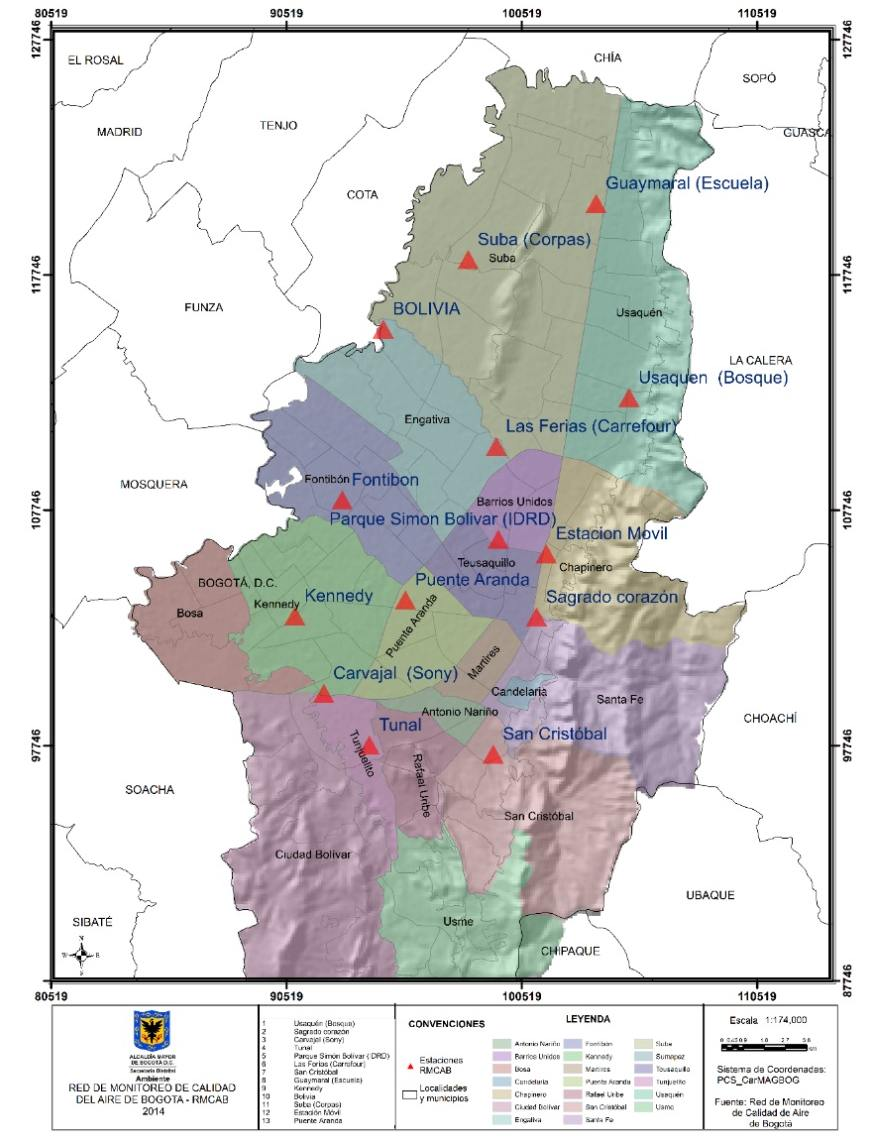
\includegraphics[scale=0.20]{Ubicacion_RMCAB}\end{center}}
& Guaymaral & Fontibón\\\\
& Usaquén & Puente Aranda  \\\\
& Suba & Kennedy \\\\
& Bolivia & Carvajal \\\\
& Las Ferias & Túnal \\\\
& P. Simón Bolívar & San Cristóbal \\\\
& Sagrado corazón & Móvil \\\\
\hline
\hline
\end{tabular}
\\\textbf{Fuente:} http://ambientebogota.gov.co/red-de-calidad-del-aire
\label{tabla:RMCAB}
\end{table}

\begin{table}[!htbp]
\begin{center}
\caption{Tabla Clasificación Variables RMCAB.}
\resizebox{10cm}{!} {
\begin{tabular}{|l|l|}
\hline
Concentraciones Atmosféricas & Fenómenos  Meteorológicos \\
\hline \hline
Óxidos de Nitrógeno & Precipitación \\ \hline
Dióxido de Azufre & Temperatura \\ \hline
Material Particulados en sus Fracciones Total & Radiación Solar \\ \hline
Material Particulados en sus Fracciones Respirable & Velocidad del Viento \\ \hline
Material Particulados en sus Fracciones Fina & Dirección del Viento \\ \hline
Ozono & Presión Barométrica \\ \hline
Monóxido de Carbono & Húmedad Relativa \\ \hline
Metano &  \\ \hline
Benceno &  \\ \hline
Tolueno &  \\ \hline
Formaldehído &  \\ \hline
Hidrocarburos No Metánicos & \\ \hline
\end{tabular}
}
\label{tabla:variables RMCAB}
\\\textbf{Fuente:} http://ambientebogota.gov.co/red-de-calidad-del-aire
\end{center}
\end{table}


\begin{center}
\chapter{METODOLOGÍA}\label{cap.metodologia}
\end{center}
\section{Resumen}
Para el desarrollo de la investigación y la aplicación de la arquitectura segura computacional, se debía contar con la información o datos a utilizar en el experimento,estos datos obtenidos de diferentes fuentes de información, de esta manera se realizaron las diferentes solicitudes, descargar y archivo de la datos de las tres fuentes como son Hospital del Sur, Secretaría de Medio Ambiente de Bogotá y el Instituto Nacional de Salud.Luego de obtener los datos requeridos, se deberá estructurar el desarrollo de la investigación en dos ramas, como es la minería de datos o explotación de información enfocados hacia la metodología CRISP-DM (Cross Industry Standard Process for Data Mining)  y la seguridad de los datos, ya que son los pilares de la investigación. Cada rama tendrá sus ramificaciones requeridas para la necesidad de cumplir los objetivos planeados anteriormente.

\section{Minería de Datos}

	\subsection{Recolección de Datos}
    Para la investigación, salvaguardar la integridad de la información es el objetivo dentro de un proceso de minería de datos, aplicando las técnicas escogidas de cifrado combinadas a las técnicas de minería de datos esperando obtener los mejores resultados, que se verán reflejados en la fase de comparación de los datos cifrados contra los datos originales, en las mismas condiciones de minería de datos.
    
Los procesos de recopilación y recolección de la información requerida, fue de la siguiente manera:
\begin{enumerate}
	\item \textbf{Fuente: Secretaría de Ambiente Distrital:} La base de datos requerida para la investigación, es la Red de Monitoreo de Calidad del Aire de Bogotá, en cual se registran las variables meteorológicas y ambientales respecto a la contaminación de aire. Actualmente se encuentran 13 estaciones de monitoreo, de las cuales doce son fijas y una móvil. La información se solicitó formalmente con los Radicados SDA No. 2016ER142305, 2016ER142728, 2016ER143626 del 18/08/2016 y 2016ER142929, 2016ER142733 del 19/08/2016, en el cual se obtuvo respuesta el día 29 de Agosto del año 2016. Donde nos especifican la información técnica de cada estación y dos direcciones IP para el acceso y descarga de la información que se requiera.c
    \begin{itemize}
		\item %http://201.245.192.252:81/App_Files/Hojas_de_Vida_Estaciones_2014\%20\%28carpeta\%29.pdf
        \item http://201.245.192.252:81
	\end{itemize}
    \item \textbf{Fuente: Hospital del Sur:} La información  que se  obtiene para esta investigación es proveniente de fuentes de información externa, recopilada a través de un acceso al servidor del Instituto Nacional de Salud Colombiano, que se ingresa de la siguiente manera:
    \begin{enumerate}
		\item Abrir una hoja de cálculo (excel, openoffice).
        \item Buscar la opción de Fuentes externas, escogiendo el método de conexión Analysis Services, que crea una coexión a un cubo de SQL Server Analysis Service a través de una tabla dinámica.
        \item Se ingresar los siguientes datos:
            \begin{itemize}
				\item \textbf{Nombre del Proveedor:} cubos.sispro.gov.co
       			 \item \textbf{Usuario:} sispro.local\textbackslash usuario1
				\item \textbf{Contraseña:} usuario1
	\end{itemize}
    	\item Escoger el tipo de acceso directamente al cubo del Sispro o de Servicios Públicos.
        \item Ya para el usuario, escogerá los filtros a utilizar según los datos o columnas que se requieran.
	\end{enumerate}
    

    \item \textbf{Fuente: Instituto Nacional de Salud:} La información tiene el mismo origen del Hospital del Sur y el mismo método de acceso al anterior.
\end{enumerate}

\subsection{Modelo de Minería de Datos}

Para el tratamiento de los datos con los que se cuenta y a los que se tiene acceso de manera permanente, es necesario no solo contar con toda si no también tener la capacidad de organizarlos a través de un método de minería de datos agrupados y de manera no jerárquicos con lo que se garantiza una uniformidad en los datos para para proceder a ser analizados por medio de la herramienta Rapidminer,es evidente que la información debe ser protegida, pero también explotada.En la agrupación de los datos se contara con una serie de elementos  con un criterio de cercanía ,información de datos no agrupados,y que buscan tener orden  para determinar su prioridad.

\begin{figure}[htb]
\centering
\caption{Fases del modelo de proceso CRISP-DM.} 
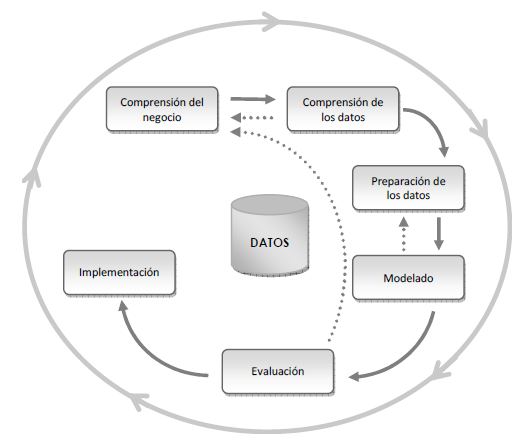
\includegraphics[scale=0.50]{CRIPS}
\\\textbf{Fuente:} http://www.crisp-dm.org/
\label{fig:Ubicacion}
\end{figure}

\begin{enumerate}
	\item \textbf{Como preparación de datos:}
    \begin{enumerate}
		\item Evaluar los datos recibidos (atributos,datos importantes,datos faltantes).
    	\item Verificar que existan los datos suficientes para dicha investigación que cubran todas las variables de interés dentro de cada uno de sus atributos.
    	\item Verificar la necesidad de que estos datos sean anonimizados para obtener pruebas y los diferentes resultados finales.
	\end{enumerate}
    \item \textbf{Como selección de datos:}
    \begin{enumerate}
		\item Caracterizar las variables tanto de entrada como de salida y conocer su nivel de importancia dentro de cada una de las bases de datos,tanto los RIPS como SIVIGILA y el RMCAB.
    	\item Identificar el tipo de algoritmo o técnica a realizar de minería de datos.
	\end{enumerate}
    \item \textbf{Dar a conocer un modelo inicial:}
     \begin{enumerate}
		\item En cuanto a lo descriptivo para dar a entender el por que se realizo la minería de datos, de clasificación si se realiza minería para clasificar y finalmente de predicción.
    	\item Dar forma al modelo realizado describiendo  los resultados encontrado sobre la situación actual.
	\end{enumerate}
    \item \textbf{Implementar el modelo:}
      \begin{enumerate}
		\item Revisar los atributos que fueron tomados finalmente para la minería y preparar su respectiva justificación.
    	\item Dar a conocer los resultados finales.
	\end{enumerate}
\end{enumerate}

\section{Perturbación}
Inicialmente en el proceso del cifrado de la información, se aplicará el método de perturbación a los datos tipo médico en la base de datos del Hospital del Sur, el resultado de dicho método será la anonimización de la información para el instante de querer publicar los datos a entes ajenos al hospital.

Para garantizar la confidencialidad a la información suministrada por las fuentes nombradas anteriormente, se abordará a través del algoritmo AES para el cifrado y descifrado de los datos. Se generará una llave privada de tamaño 128, 192 ó 256 bits. Este método evita que la llave privada se catalogue como débil o semi - débil\footnote{PENCHALAIAH PhD, SESHADRI  PhD. Effective Comparison and Evaluation of DES and Rijndael Algorithm (AES), International Journal on Computer Science and Engineering Vol. 02, No. 05, 2010, 1641-1645 Pág. 1642.} dentro de la clasificación de tipos de claves.
    
    \subsection{Perturbación de Datos}
     Para garantizar la confidencialidad de la información en la base de datos del Hospital del Sur, debemos aplicar el método de anonimización a ciertas columnas o datos (carácter médico o personal), de esta manera se aplicará la técnina de pertubación (micro agregación de datos) a los datos originales. La perturbación se realizará a partir de la distribución normal o gausiana a datos númericos, la cual es la distribución de probabilidad normal de variables aleatorias, donde esta se pueden aproximar a una distribución normal. \footnote{ÁNGEL A. Juan, SEDANO Máximo, VILA Alicia.} %<http://www.uoc.edu/in3/emath/docs/Distrib_Normal.pdf> [citado en Septiembre 18 del 2016] Pág. 3 }. 
Mientras a los datos tipo String, se aplicará el intercambio aleatorio de los datos.

Los pasos a seguir en esta fase serán:
\begin{enumerate}
	\item Selección de los datos a perturbar de las tres bases de datos, justificando su selección y el método a aplicar.
    \item Desarrollo de los Scripts en código Python, para la investigación se realizará utilizando Sublime Text 2 como editor de código.
    \item Ejecución de los scripts anteriores desde consola, utilizando Anaconda\footnote{https://www.continuum.io/downloads} como herramienta para ejecución de archivos de extensión .py.
    \item Verificación de la correcta ejecución de los script tomando las correcciones pertinentes en caso que no sean los resultados esperados.
\end{enumerate}

	 \subsection{Protocolo SSL}
     Aprovechando las propiedades del protocolo SSL para el envió y recepción de los datos o archivos entre las partes, se aplicará este protocolo ya que garantiza la confidencialidad e integridad de la información. La comunicación de las entidades, por su ubicación geográfica diferente y lejana, se utilizará el Internet como medio de comunicación entre los servidores de las tres entidades involucradas en la investigación; el protocolo SSL permitirá cifrar la información desde el servidor origen para enviar a los otros dos servidores para su debido descifrado. Se debe tener en cuenta que la información enviada implementado el protocolo SSL será de datos o archivos perturbados y cifrados, generando a través del protocolo la llave privada (para cifrar) y pública (descifrada y enviada por certificación digital).\\\\
Los pasos para la implementación del protocolo SSL, será dado por:
\begin{enumerate}
	\item Búsqueda e instalación de OpenSSL Versión 1.1.0 actualmente estable \footnote{https://www.openssl.org/source/} (herramienta para la implementación del Protocolo SSL) de maneral local.
    \item Instalación de OpenSSL en otro computador para pruebas de comunicación y envió de la información.
    \item Ejecución del Protocolo mediante OpenSSL entre los dos computadores.
    \item Verificar los resultados esperados tomando las correcciones pertinentes al protocolo.
\end{enumerate}

     \section{Comparación Datos Cifrados - Originales}
En esta fase se tendrá en cuenta los resultados de los dos procesos de minería de datos aplicados, donde se debió realizar los siguientes pasos en resumen para llegar a esta etapa de la investigación:
\begin{enumerate}
	\item Minería de Datos a la información original sin perturbación o alteración alguna.
    \item Perturbación - anonimización de los datos originales seleccionados de las bases de datos.
    \item Minería de Datos a la información perturbada - anonimizada con los mismos pasos del paso N.01.
    \item Envió de la información a través del protocolo SSL utilizando OpenSSL.
    \item Comparacaión y análisis de los dos resultados de minería de datos (Originales - Perturbados).
\end{enumerate}

\begin{center}
 \chapter{MARCO DE REFERENCIA}\label{cap.referencia}
\end{center}

\section{MARCO TEÓRICO}

Las Infecciones Respiratorias Agudas (IRA) constituyen un grupo de enfermedades que se producen en el aparato respiratorio, causadas por diferentes microrganismos como virus y bacterias, que comienzan de forma repentina y duran menos de 2 semanas aproximadamente. Es una de las infecciones más frecuente en el mundo y representa un importante tema de salud pública en nuestro país.  La mayoría de estas infecciones como el resfriado común son leves, pero dependiendo del estado general de la persona pueden complicarse y llegar a amenazar la vida, como en el caso de la neumonía.\\\\
En niños menores de 5 años, la causa de la infección en el  95\% de los casos son los virus siendo de buen pronóstico, pero un pequeño porcentaje puede padecer complicaciones como  otitis, sinusitis y neumonía. Unos de los efectos que generan gran impacto a nivel local son  la combustión y efectos de cambio climático. Por esto  gran parte de la ciudad adelanta campañas con las que promueve la mejora de la calidad del aire, que con el tiempo será vital.\\\\
Se afirma que en países en desarrollo, del 2 al 3\% de los niños presentan enfermedades como neumonía. En invierno es cuando incrementa más la posibilidad de infección viral y también afecta a las mujeres embarazadas y a personas con enfermedades respiratorias.\\\\
Como parte fundamental tambien se encuentra la manera de obtener dichos datos En cuanto al proceso inicial de los procesos de extracción, transformación y carga (ETL), esto constituye un aspecto clave para llevar a buen camino la integración de los datos, cuyo principal objetivo es conseguir un óptimo rendimiento en la obtención de datos de calidad, que respondan a las necesidades de la empresa de forma fiable.\\\\
La minería de datos se define como el proceso de exploración y análisis, por medios automáticos o semiautomáticos, de grandes volúmenes de información con el objetivo de descubrir e identificar patrones y reglas
significativas\footnote{M. Berry, G. Linoff, “Mastering data mining: the art andscience of customer relationship management“. West Susex:John Wiley \& Sons, 1999}.De manera clara se requiere no solo una tecnica de mineria de datos si no también una metodología de trabajo,como lo es la CRISP-DM de esta manera surge la necesidad de contar con una herramienta que permita evaluar y confrontar las diferentes 




Dentro del agrupamiento de los datos almacenados, el objetivo principal es encontrar que los objetos de un grupo sean similares entre sí y diferentes de los objetos de otros grupos, aplicando clusters (Colección de métodos Estadísticos).\\\\
Es por esto que tanto los  RIPS, SIVIGILA, RMCAB y demás entes que permitieron la recopilación de esta información serán de vital importancia para toda la investigación llevada a cabo. En cuanto a la contaminación en el aire, como principal eje de este factor de riesgo ambiental, analizar qué impacto tiene localmente (Bogotá D.C). De esta manera se tendrá una interacción entre los datos clínicos y la ejecución de métodos computacionales que arrojarán resultados para obtener una serie de análisis y unas conclusiones luego de su proceso. Componente importante dentro de estos procesos sera el de ETL donde se tendrá en cuenta la agrupación de datos para realizar clasificación de grupos basados en su similaridad. \\\\
De esta manera surge la arquitectura multi-partita computacional o  Secure Multiparty Computation (SMC) que permite que entidades o datasets tengan sus entradas independientes para alimentar procesos intermedios para generar salidas independiente, cuidando la comunicación segura de las entradas\footnote{DAMGARD Ivan, et at. Multiparty Computation from Somewhat Homomorphic Encryption, International Association for Cryptologic Research 2012, R. Safavi-Naini and R. Canetti (Eds.): CRYPTO 2012, LNCS 7417, pp. 643.} pero ademas, permitiendo compartir trozos o subconjuntos de datos autorizados con otros participantes\footnote{GHODOSI Hossein Ghodosi, et at. Multi-party computation with conversion of secret sharing, Springer Science+Business Media, LLC 2011, Des. Codes Cryptogr. (2012) 62:259–272, Online: 10 May 2011,pp. 260.}. Una expectativa en el proceso SMC es la interacción entre las partes que permita una funcionalidad independiente pero relacionada para compartir información de manera segura y protegiendo la confidencialidad de cada dato\footnote{KIRAZ SABIR Mehmet, UZUNKOL Osmanbey. Efficient and verifiable algorithms for secure outsourcing of cryptographic computations, Springer-Verlag Berlin Heidelberg 2015, Int. J. Inf. Secur, Online: 15 Nov 2015,pp. 1.}.  \\\\
Dentro de la arquitectura multi-partita existe gran variedad de técnicas para garantizar la seguridad en este protocolo, como son circuitos ilegibles (garbled circuits), compartiendo secretos (secret sharing) o cifrado homomórfico (homomorphic encryption)\footnote{LAUD Peeter. Privacy-Preserving Minimum Spanning Trees through Oblivious Parallel RAM for Secure Multiparty Computation, Online: 25 Nov 2014,pp. 3.}. Así, la preservación de la privacidad se obtendrá aplicando la técnica según se requiera. Dentro de las técnicas nombradas se vincula dentro de una composición de una caja negra aritmética (ABB)\footnote{ibi, p. 5.}.

\textbf{\textit{Criptografía:}}

En la actualidad los bancos para los procesos de cifrado y descifrado, están trabajando bajo el estándar de encriptación avanzado AES (Advanced Encriyption Standard), en cual la relación entre el consumo computacional y la seguridad que debe garantizar es muy importante, pero en este caso existe un equilibrio para poder trabajar bajo el estándar nombrado. Se debe tener en cuenta los fundamentos generales de la criptografía, donde existe tres campos de acción en el momento cifrar o proteger cualquier información Cuadro 3.1: 

\begin{table}[ht]
\centering
\caption{Conceptos Generales Cifrados.}\footnote{GOMEZ Vieitis Alvaro. Sistema seguros de acceso y transmisión de datos, RA-MA Editorial Pag 15.}
\begin{tabular}{>{\centering\arraybackslash}m{3cm} >{\arraybackslash}m{9cm} }
\hline
\textbf{\textit{Conceptos:}} & \textbf{\textit{Definición:}} \\ \hline
Criptografía & "...es la ciencia que se encarga de estudiar las distintas técnicas empleadas para transformar (“encriptar” o “cifrar”) la información y hacerla irreconocible a todos aquellos usuarios no autorizados de un sistema informático, de modo que solo los legítimos propietarios puedan recuperar (“desencriptar” o “descifrar”) la información original..." \\ \hline
Criptoanálisis & "...es la ciencia que se ocupa de estudiar herramientas y técnicas que permitan romper los códigos y sistemas de protección definidos por la criptografía...." \\ \hline
Criptología & "...es la ciencia de inventar sistemas de cifrado de la información (criptografía) y de desbaratarlos (criptoanálisis) se la conoce colectivamente con el término de Criptología . ..." \\ \hline
\end{tabular}
\label{tabla:ConceptosCriptograficos}
\\\textbf{Fuente:} GOMEZ Vieitis Alvaro. Sistema seguros de acceso y transmisión de datos, RA-MA Editorial.
\end{table}

Además se debe tener en cuenta que los sistemas criptográficos, pueden ser objetos de ataques, para robo o alteración de la información que se esta protegiendo y dando confidencialidad, de esta manera según el criptoanálisis se puede clasificar en 4 tipos, los cuales son:

\begin{enumerate}
	\item \textbf{Ataques basados solo en el texto cifrado:}  se tiene varios textos protegidos con el objetivo de encontrar la clave y recuperar la información original (fuerza bruta).\footnote{ibi, p. 21}
    \item \textbf{Ataques basados en texto claro conocido:} se tiene varios textos o información cifrados, los cuales se utilizarán para descifrar y encontrar la llave en otros textos.\footnote{ibi, p.  21}
    \item \textbf{Ataques basados en texto claro seleccionado:} similar al proceso anterior, pero en este caso se selecciona los textos cifrados con características similares para descifrar y encontrar la clave en otros textos cifrados.\footnote{ibi, p. 21}
    \item \textbf{Ataques adaptativos basados en texto claro conocido: } con procesos de cifrados anteriores, se busca la estrategia de modificar aquellos procesos por parte para ir aplicando la modificación sobre los textos cifrados objetos para descifrado.\footnote{ibi, p. 21}
\end{enumerate}

De la clasificación de los sistemas criptográficos, dependerá del orígen o naturaleza de las llaves de cifrado / descifrado Fig. 3.1, donde existe los procesos simétricos y asimétricos, donde los primero tienen la misma llave para cifrar y descifrar, mientras que el segundo se genera dos llaves diferentes pero relacionadas entre sí, una para cifrar y otra para descifrar durante el proceso de cifrado. Después de aplicar el sistema de cifrado, la información se debe complementar también de algunas condiciones para garantizar plenamente la confidencialidad y seguridad de los textos u objetos cifrados. Estas condiciones serán dadas por la robustez del esquema de cifrado diseñado y la adecuada gestión de las claves.

\begin{figure}[htb]
\centering
\caption{Clasificación de los sistemas criptográficos.}\footnote{GOMEZ Vieitis Alvaro. Sistema seguros de acceso y transmisión de datos, RA-MA Editorial Pag 23}
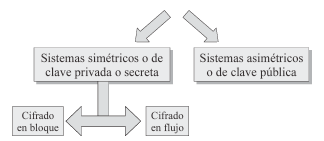
\includegraphics[scale=0.8]{ClasificacionCripto}
\label{fig:ClasificacionCripto}
\\\textbf{Fuente:} GOMEZ Vieitis Alvaro. Sistema seguros de acceso y transmisión de datos, RA-MA Editorial.
\end{figure}

En el momento de definir de la robustez del esquema, se debe definir a través de métricas tres propiedades primordiales en el algoritmo aplicado, ya que una demostración matemática del algoritmo en general es difícil; donde las propiedades son de confusión, difusión y completitud.\footnote{ibi, p. 38} Cuadro. 3.2.\\\\
Pero es realmente difícil poder aplicar un algoritmo con grados altos de las propiedades nombradas, ya que también se debe garantizar el buen uso de los servicios y recursos computacionales, trabajando en conjunto con la comunicación para envió y recepción de la información cifrada. Teóricamente el único sistema irrompible es el propuesto en 1917 por Gilbert Vernam (Cifrado de Vernam one - time pad) donde con una sola clave que se genera de manera aleatoria y del mismo tamaño del mensaje a cifrar, solamente se dará al impostor la longitud del mensaje, agregando que solo se podrá utilizar una vez dicha clave.

\begin{table}[ht]
\centering
\caption{Propiedades de Robustez en el esquema diseñado de cifrado.}\footnote{GOMEZ Vieitis Alvaro. Sistema seguros de acceso y transmisión de datos, RA-MA Editorial Pag 38.}
\begin{tabular}{>{\centering\arraybackslash}m{3cm} >{\arraybackslash}m{10cm} }
\hline
\textbf{\textit{Conceptos:}} & \textbf{\textit{Definición:}} \\ \hline
\textbf{\textit{Confusión:}} & "...permite ocultar la relación entre el texto claro y el texto cifrado, dificultando el análisis de patrones estadísticos (se consigue generar la "confusión" mediante operaciones de sustitución de símbolos)..." \\ \hline
\textbf{\textit{Difusión:}} & "...pretende disimular las redundancias del texto claro al extenderlas por todo el texto cifrado (característica que se consigue gracias a las operaciones de transposición de símbolos)...." \\ \hline
\textbf{\textit{Completitud:}} & "...se cumple si cada bit de texto cifrado depende de todos y cada uno de los bits de la clave. En otro caso, se podrían realizar ataques contra determinadas partes de la clave, en una estrategia de “divide y vencerás”..." \\ \hline
\end{tabular}
\label{tabla:RobustezPropiedades}
\\\textbf{Fuente:} GOMEZ Vieitis Alvaro. Sistema seguros de acceso y transmisión de datos, RA-MA Editorial.
\end{table}

Pero desde el punto práctico un sistema criptográfico, se puede medir frente a los ataques de fuerza bruta (se explora todas las posibilidades de claves dentro del rango del sistema criptográfico),  ataques de diccionarios (trabajar con una lista de posibles claves alimentadas de fuentes de información, de la organización dueña de la información) y contra la implementación del algoritmo.\footnote{ibi, p. 39}\\\\
Ya para la adecuada gestión de claves, ya que se debe definir muy bien los roles de las personas que tengan las claves y los tipos de acceso de la información. Donde la tecnología criptográfica se encuentra sometida a la regulación de la norma International Traffic in Arms Regulations (ITAL)\footnote{ibi, p. 41} ya que se cataloga de peligro por el manejo de información cifrada que los gobiernos no puedan descifrar.\\\\
\textbf{Perturbación}\\\\
Pero no solamente cifrando la información se podrá dar garantía de confidencialidad de los datos, ya que las personas o entidades que obtengan las claves para descifrar, podrán acceder a la información original. De esta manera existen varios procesos o técnicas de anonimización de la información, done es la modificación sistemática de datos, lo cual causará que no sean precisas para revelar o identificar registros individuales puntuales \footnote{Dirección de Regulación, Planeación, Estandarización y Normalización DIRPEN. Lineamientos para
la Anonimización de microdatos VERSIÓN: 01 29-08-2014 Pág. 19}.\\\\
Algunos de los métodos de anonimización actuales, se basan en la modificación parcial de los valores de los datos (métodos de perturbación) o cambio de posición de los mismos (métodos de reducción de datos), igualmente se relacionarán a continuación según la tabla N. 3.3 y 3.4: 

\begin{table}[ht]
\centering
\caption{Técnicas de Anonimización basados en la perturbación de datos.}
\begin{tabular}{>{\centering\arraybackslash}m{3cm} >{\arraybackslash}m{10cm} }
\hline
\textbf{\textit{Conceptos:}} & \textbf{\textit{Definición:}} \\ \hline
\textbf{\textit{Micro - agregación:}} & Es reemplazar un valor observado con la media calculada sobre un pequeño grupo de unidades para agregarlos a los datos a perturbar. \\ \hline
\textbf{\textit{Agrupación:}} & Los registros contenidos en el conjunto original se agrupan en subconjuntos de cardinalidad; por lo menos k mediante algún criterio de similitud.\\ \hline
\textbf{\textit{Sustitución:}} & Cada registro del conjunto original es substituido por el registro medio del subconjunto al cual ha sido asignado en la etapa anterior. \\ \hline
\textbf{\textit{Intercambio aleatorio de datos - PRAM (Post Randomization Method):}} & Es un método de control de la difusión estadística que se puede aplicar a los datos categóricos \\ \hline
\textbf{\textit{Distorsión de datos por una distribución de probabilidades:}} & Se pretende obtener un conjunto de datos protegido aleatoriamente a partir del conjunto de datos original \\ \hline
\end{tabular}
\label{tabla:RobustezPropiedades}
\\\textbf{Fuente:} Lineamientos para la anonimización de datos del sistema nacional de estudios y encuestas poblacionales para la salud Ministerio de Salud Y Protección Social Dirección de Epidemiología e Demografía de Colombia.
\end{table}

\begin{table}[htbp]
\centering
\caption{Técnicas de Anonimización basados en la reducción de datos.}
\begin{tabular}{>{\centering\arraybackslash}m{3cm} >{\arraybackslash}m{10cm} }
\hline
\textbf{\textit{Conceptos:}} & \textbf{\textit{Definición:}} \\ \hline
\textbf{\textit{Eliminación de variables:}} & La primera aplicación de este método es la eliminación de identificadores directos desde el archivo de datos. \\ \hline
\textbf{\textit{Eliminación de registros:}} & Esta técnica consiste en eliminar un registro completo, pero esta alterada los resultados estadísticos lo cual se debe evitar aplicar.  \\ \hline
\textbf{\textit{Recodificación global:}} & Combina categorías para formar nuevas categorías menos específicas. \\ \hline
\end{tabular}
\label{tabla:RobustezPropiedades}
\\\textbf{Fuente:} Lineamientos para la anonimización de datos del sistema nacional de estudios y encuestas poblacionales para la salud Ministerio de Salud Y Protección Social Dirección de Epidemiología e Demografía de Colombia.
\end{table}

En las características del cifrado AES, para el cifrado avanzado de la información se compara con otro algoritmo como es DES, el anterior inmediato al AES, donde dicho algoritmo según el tamaño de claves o llaves, genera un número determinado de llaves:
\begin{itemize}
	\item 128 bits: aproximadamente 3,4 x 1.038 posibles claves\footnote{PENCHALAIAH PhD, SESHADRI  PhD. Effective Comparison and Evaluation of DES and Rijndael Algorithm (AES), International Journal on Computer Science and Engineering Vol. 02, No. 05, 2010, 1641-1645 Pág. 1642.}.
    \item 192 bits: aproximadamente 6.2 x 1.057 posibles claves\footnote{ibi p. 1642.}.
    \item 256 bits: aproximadamente 1,1 x 1077 posibles claves\footnote{ibi p. 1642.}.
\end{itemize}

De esta manera, la investigación implementará el algoritmo AES de longitud 128 bits dentro del protocolo SSL, donde la comparación con la longitud de DES de 56 bits, donde este se genera 7,2 x 1016 posibles claves, con una diferencia en magnitud de 1021 claves más\footnote{ibi p. 1642.}. Este algoritmo es la última tendencia en el área de seguridad informática en los bancos, entes gubernamentales y de seguridad nacional. Sí se quisiera romper la clave generará por el algoritmo DES teóricamente en un segundo con una máquina de 149 mil millones de dólares para romper una clave AES se tardaría 149 billones de años con una longitud de 128 bits\footnote{ibi p. 1642.}.\\\\
\textbf{Protocolo SSL}\\\\
Ya definido la manera de cifrar y anonimizar la información, se debe definir el método o técnica de envió de los datos cifrados y perturbados. El protocolo para aplicar en la investigación sera el SSL (Secure Sockets Layer)  el cual provee privacidad y confiabilidad a la comunicación entre dos partes o aplicaciones. El enlace que se genera entre las dos partes es cifrado, donde garantizará la privacidad e integridad de los datos\footnote{ SSL Information and FAQ [En línea] <http://info.ssl.com/article.aspx?id=10241> [citado en 18 de Septiembre del 2016]}\\\\
El protocolo SSL esta diseñado para autenticar el emisor y receptor, así mismo salvaguardar la confidencialidad e integridad de la información. Para el envió de los datos entre las partes, se genera una llave privada para cifrar los datos o archivos, pero es conservada por el emisor de esta manera al querer descifrar se aplica una llave pública por el emisor por medio de un certificado \footnote{Utilizar el protocolo SSL <http://www.4d.com/docs/CMS/CMS02064.HTM> [En línea] [citado en 18 de Septiembre del 2016]} de tipo X.509. El uso de este protocolo es amplio ya que se puede implementar en  navegación web, correo electrónico, fax por Internet, mensajería instantánea, y voz-sobre-IP (VoIP).\\\\
El certificado digital permitirá garantizar la identidad de las partes, el cual el objetivo de este certificado es asociar una clave pública con la identidad del usuario contenida en el certificado\footnote{SEJWANI Sapna, TANWAR Sarvesh, Implementation of X.509 Certificate for Online Applications, International Journal of Research in Advent Technology, Vol.2, No.3, March 2014, E-ISSN: 2321-9637, Pág. 250} pero se debe tener en cuenta que la seguridad para la autenticación online dependerá de la integridad de la llave pública, ya que sí un atacante logra reemplazar la llave pública con la suya, podrá acceder a los datos confidenciales o protegidos\footnote{ibi p. 250.} pero este ataque se evita generando una firma digital de una autoridad de certificación, donde la firma es un resumen del mensaje de todos los campos del certificado codificados con la clave privada de la entidad emisora\footnote{ibi p.250.}.\\\\
\textbf{Arquitectura Descentralizada}\\\\
\section{ESTADO DEL ARTE}
	\subsection{Seguridad}
Para el envió de los datos se tendrá en cuenta la seguridad informática aplicada al estudio de investigación, se plantea una comunicación entre las partes sin tener en cuenta el costo computacional, simulando bases de datos privadas y públicas\footnote{KIRAZ SABIR Mehmet, UZUNKOL Osmanbey. Efficient and verifiable algorithms for secure outsourcing of cryptographic computations, Springer-Verlag Berlin Heidelberg 2015, Int. J. Inf. Secur, Online: 15 Nov 2015,pp. 2.}. En el caso de la investigación, cada dataset será clasificada como privada para realizar un proceso ETL y de esta manera diseñar una base de datos público para realizar la minería de datos. La inserción de los datos entre la base de datos para el procesamiento computacional se realizará entre las partes con datos cifrados\footnote{ibi, p.  4.}.\\\\
De esta manera se diseñará una arquitectura flexible basado en la conversión de compartir secretos de las bases de datos privadas para realizar la minería de datos en una base pública, donde se tendrá en cuenta el nivel de complejidad de los datos a extraer de cada dataset según el número de participantes, de esta manera los datos extraídos serán catalogados como partes de secretos de su origen\footnote{GHODOSI Hossein Ghodosi, et at. Multi-party computation with conversion of secret sharing, Springer Science+Business Media, LLC 2011, Des. Codes Cryptogr. (2012) 62:259–272, Online: 10 May 2011,pp. 263.}.\\\\
Se debe tener en cuenta que no se cifrará toda la información, ya que las fuentes de información son instituciones públicas, solamente se dará protección a los datos de personas y ubicación de los registros de los RIPS. Figura 3.2.

\begin{figure}[htb]
\centering
\caption{Modelo Base para la Arquitectura} 
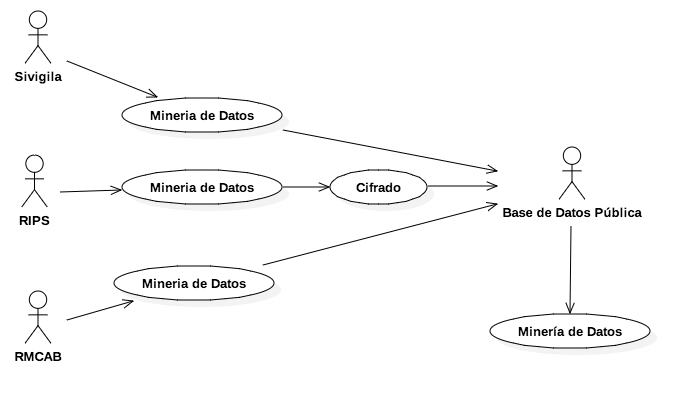
\includegraphics[scale=0.4]{Diagrama_Arq}
\label{fig:Cifrado}
\\\textbf{Fuente:} Propia.
\end{figure}

El procedimiento para el debido funcionamiento de cifrado en el sistema, se manejará el procedimiento Seguro para Transferencia de un Archivo de Datos usando Técnicas Criptográficas (simétricas )dotadas de una clave secreta AES y una clave privada RSA, ya que esta transferencia nos permitirá:

\begin{itemize}
\item Autenticación del funcionamiento del Emisor que envía la información. La firma digital obtenida a través de la clave privada RSA es imposible de falsificar.\footnote{CELINA Drovandi. CRIPTOGRAFÍA
SEGURIDAD EN ESQUEMAS DE FILE TRANSFER SEGURIDAD EN INTERNET Revista de la Universidad de Mendoza, 2015 pag 374}
\item Confidencialidad, ya que los datos encriptados no pueden ser interpretados por nadie que no esté autorizado por el Receptor.\footnote{ibid, p. 374.}
\item Integridad de la Información: cualquier alteración, ya sea accidental o maliciosa de los datos, por mínima que sea, hará que en el proceso de desencriptado la información no resulte clara sino que se transforme en un conjunto ilegible de caracteres.\footnote{ibid, p. 374.}
\item Seguridad: nadie podrá enviar mensajes falsos intentando usurpar la identidad de un Emisor, ni desde adentro ni desde afuera del sistema.\footnote{ibi, p. 374.}
\item No repudio de origen y destino.\footnote{ibid, p 374.}
\end{itemize}

AES (Advanced Encryption Standard) Se basa en varias sustituciones , permutaciones y transformaciones lineales, este método es el preferido en procesos de seguridad en los estados, bancos y sistemas de alta seguridad\footnote{Dr. Bhadresh P. Patel, Vishal R. Pancholi. Enhancement of Cloud Computing Security with Secure Data Storage using AES IJIRST –International Journal for Innovative Research in Science and Technology Volume 2 Issue 09 February 2016 ISSN (online): 2349-601 Pag 18}. Una ventaja en el desarrollo del AES permite elegir un vario tipo de bits como de 128 bits, 192 bits o clave de 256 bits, por lo que es exponencialmente más fuerte que la clave de 56 bits de DES\footnote{ibi, p. 19}. Además el proceso de AES comparándolo con DES y RSA, es mejor ya que consumen menos tiempo de cifrado pero mucho mayor de intento de descifrado anormal\footnote{ibi, p. 19}.  

El proceso de cifrado AES se compone de una serie de operaciones vinculadas , algunos de los cuales implican la sustituciones específicas y otros implican alrededor de los bits (permutaciones)\footnote{ibi, p.  20} Figura 3.3. 

\begin{figure}[htb]
\centering
\caption{Cifrado y descifrado en AES} 
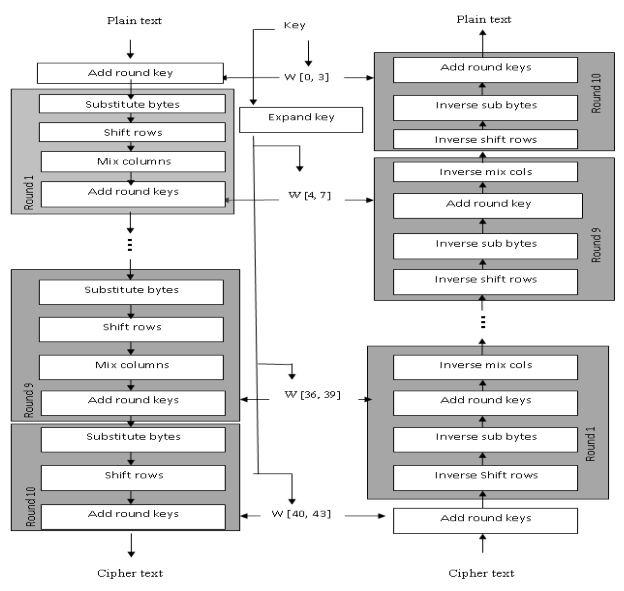
\includegraphics[scale=0.3]{AES}
\label{fig:CifradoAES}
\\ \textbf{Fuente:} Dr. Bhadresh P. Patel, Vishal R. Pancholi. Enhancement of Cloud Computing Security with Secure Data Storage using AES IJIRST –International Journal for Innovative Research in Science and Technology Volume 2 Issue 09 February 2016 ISSN (online): 2349-601.
\end{figure}

El cifrado AES actualmente se esta implantando e implementando en las tecnologías actuales de la nube, ya que es el método más rápido que tiene la flexibilidad y capacidad de ampliación, consumiendo poca memoria a comparación de los otros métodos de cifrado simétrico. En términos de resistencia contra una variedad de ataques tales como ataque cuadrado, clave de ataque, ataque clave de recuperación y el ataque diferencial. Por lo tanto, el algoritmo AES es un método de cifrado de alta seguridad. Los datos también puede proteger contra ataques futuros, tales como ataques de la rotura violenta\footnote{ibi, p. 21}. En la actualidad la mayor parte de los algoritmos criptográficos son públicos y se basan en una serie de operaciones elementales sobre los datos que constituyen el texto original: transposiciones (cambiar el orden de los símbolos que forman parte del texto) y sustituciones  (reemplazar unos símbolos por otros)\footnote{GOMEZ Vieitis Alvaro. Sistema seguros de acceso y transmisión de datos, RA-MA Editorial Pag 17}.

Para la implementación del protocolo SSL, se utilizará el recurso de OpenSSL \footnote{https://www.openssl.org} el cual es un proyecto de caracter de desarrollo libre en C desarrollado por Eric Young y Tim Hudson. Esta herramienta cuenta con ser capaz de operar en los siguientes sistemas operativos como Linux y
Microsoft Windows, pero también implementando los algoritmos criptográficos que implementa son: AES, Blowfish, Camellia, SEED, CAST-128, DES, IDEA, RC2, RC4, RC5, TDES, GOST 28147-89, RSA y DSA\footnote{
VELASCO Sánchez Paola Maritza, ANÁLISIS DE LOS MECANISMOS DE ENCRIPTACIÓN PARA LA SEGURIDAD DE LA
INFORMACIÓN EN REDES DE COMUNICACIONES, FACULTAD DE INGENIERÍA MAESTRÍA EN REDES DE COMUNICACIONES, PONTIFICIA UNIVERSIDAD CATÓLICA DEL ECUADOR Año 2015 Pàg. 28}. Una caracteristica sobre saliente es que permire al sistema a implementar el Secure Sockets Layer (SSL).

Consiste en un robusto paquete de herramientas de administración y bibliotecas relacionadas con la criptografía, que suministran funciones criptográficas a otros paquetes como OpenSSH y navegadores web (para acceso seguro a sitios HTTPS).

\subsection{Minería de Datos}

La aplicación automatizada de algoritmos de minería de datos permite detectar fácilmente patrones en los datos, razón por la cual esta técnica es mucho más eficiente que el análisis dirigido a la verificación cuando se intenta explorar datos procedentes de repositorios de gran tamaño y complejidad elevada. Dichas técnicas emergentes se encuentran en continua evolución como resultado de la colaboración entre campos de investigación tales como bases de datos, reconocimiento de patrones, inteligencia artificial, sistemas expertos, estadística, visualización, recuperación de información, y computación de altas prestaciones. Los algoritmos de minería de datos se clasifican en dos grandes categorías: supervisados o predictivos y no supervisados o de descubrimiento del conocimiento\footnote{Weiss, S.M. y Indurkhya, N. “Predictive Data Mining. A Practical Guide”Morgan Kaufmann Publishers, San Francisco, 1998.}\\\\
Los algoritmos supervisados o predictivos predicen el valor de un atributo (Etiqueta) de un conjunto de datos, conocidos otros atributos (atributos descriptivos). A partir de datos cuya etiqueta se conoce se induce una relación entre dicha etiqueta y otra serie de atributos. Esas relaciones sirven para realizar la predicción en datos cuya etiqueta es desconocida. Esta forma de trabajar se conoce como aprendizaje supervisado y se desarrolla en dos fases: Entrenamiento (construcción de un modelo usando un subconjunto de datos con etiqueta conocida) y prueba (prueba del modelo sobre el resto de los datos). Cuando una aplicación no es lo suficientemente madura no tiene el potencial necesario para una solución predictiva, en ese caso hay que recurrir a los métodos no supervisados o de descubrimiento de  conocimiento que descubren patrones y tendencias en los datos actuales (no utilizan datos históricos). El descubrimiento de esa información sirve para llevar a cabo acciones y obtener un beneficio (científico o de negocio) de ellas. En la tabla siguiente se muestran algunas de las técnicas de minería de ambas categorías.

\begin{figure}[htb]
\centering
\caption{Clasificación de las técnicas de minería de datos} 
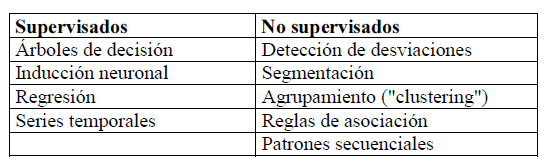
\includegraphics[scale=0.7]{Tabla1}
\label{fig:Tabla1}
\\Ingresar fuente aquí
\end{figure}

La aplicación de los algoritmos de minería de datos requiere la realización de una serie de procesos previos con el fin de  preparar los datos de entrada debido a que, en muchas ocasiones dichos datos proceden de fuentes heterogéneas que no se encuentran organizadas, no tienen el formato adecuado o
contienen ruido. Por otra parte, es necesario interpretar y evaluar los resultados obtenidos. El proceso completo consta de las siguientes etapas\footnote{Cabena, P., Hadjinian, P., Stadler, R., Verhees, J. Y Zanasi, A.
“Discovering Data Mining. From Concept to Implementation”, Prentice Hall, 1998.}:

\begin{enumerate}
\item \textbf{Preparación de Datos:}
	\begin{itemize}
		\item \textbf{Selección:} Identificación de las fuentes de información externas e internas y selección del subconjunto de datos necesario.
        \item \textbf{Preprocesamiento:} estudio de la calidad de los datos y determinación de las operaciones de minería que se pueden realizar.
\end{itemize}
\item \textbf{Transformación de datos:} conversión de datos en un modelo analítico.
\item \textbf{Minería de datos:} tratamiento automatizado de los datos seleccionados con una combinación apropiada de algoritmos.
\item \textbf{Análisis de resultados:} interpretación de los resultados obtenidos en la etapa anterior.generalmente con la ayuda de una técnica de visualización.
\item \textbf{Asimilación de conocimiento:} aplicación del conocimiento descubierto
\end{enumerate}

Aunque los pasos anteriores se realizan en el orden en que aparecen, el proceso es altamente iterativo, estableciéndose retroalimentación entre los mismos. Además, no todos los pasos requieren el mismo esfuerzo, generalmente la etapa de pre-procesamiento es la más costosa ya que representa aproximadamente el 60 \% del esfuerzo total, mientras que la etapa de minería sólo representa el 10 \% . 

Con arquitecturas de  este  tipo se ha incursionado  en  algunos gremios. En algunas oportunidades con casos fallidos  y en otros con casos exitosos. Como caso fallido se tiene  la eventualidad en la  ciudad de New York en el año 2014, cuando se recopiló la información de todos los taxistas de la ciudad por parte de la alcaldía neoyorkina. Pero una falla en el proceso de cifrado MD5 permitió que personas ajenas recuperaran información personal de los taxistas de alrededor de 173 millones de viajes realizados\footnote{DAN Goodin.Poorly anonymized logs reveal NYC cab drivers’ detailed whereabouts [En linea]. New York: Dirección URL: <http://arstechnica.com/tech-policy/2014/06/poorly-anonymized-logs-reveal-nyc-cab-drivers-detailed-whereabouts/>. [30, Marzo 2015].}, dejando en evidencia sus datos personales y las rutas con sus clientes frecuentes,  perjudicando así su privacidad. Si esta información la obtuvieran grupos criminales podrían dar seguimiento a taxistas y pasajeros.\\\\
Un caso exitoso fue el de Netflix, cuando en el año 2006 logró anonimizar la información de más de 500.000 millones de clientes junto a las preferencias de los mismos, mostrando un grado de nivel alto de seguridad y preservación de la integridad de los datos\footnote{HERNANDEZ Alexander New York taxi details can be extracted from anonymised data, researchers say [En linea]. New York: Dirección URL: <https://www.theguardian.com/technology/2014/jun/27/new-york-taxi-details-anonymised-data-researchers-warn>. [30, Marzo 2015].}.\\\\

\section{MARCO LEGAL}

\subsection{Legislación Nacional}

En Colombia la legislación vigente referente a la protección de la confidencialidad se encuentra consagrada en la Constitución Política, en su Artículo 15:\\
Todas las personas tienen derecho a su intimidad personal y familiar y a su buen nombre, y el Estado debe respetarlos y hacerlos respetar. De igual modo, tienen derecho a conocer, actualizar y rectificar las informaciones que se hayan recogido sobre ellas en los bancos de datos y en archivos de entidades públicas y privadas. En la recolección, tratamiento y circulación de datos se respetarán la libertad y demás garantías consagradas en la Constitución. La correspondencia y demás formas de comunicación privada son inviolables\footnote{De Colombia CP Constitución Política de Colombia Bogotá Colombia Leyer 1991}.

En 2012, la Ley 1581, por la cual se dictan disposiciones generales para la protección de datos personales, parcialmente reglamentada por la Ley 1377 de 2013, dispone en sus principios referentes al acceso y circulación restringida de seguridad y de confidencialidad, que el acceso a los datos se debe restringir y la información debe estar sujeta a tratamiento por parte del responsable, como lo indica en su Artículo 4:

Finalmente, en el Código Nacional de Buenas Prácticas para las Estadísticas Oficiales se hace referencia a la anonimización de los micro-datos en el principio 5:

Confidencialidad. Las entidades pertenecientes al Sistema Estadístico Nacional -SEN- deben garantizar la protección y la confidencialidad de la información con la que se producen las estadísticas oficiales, así como evitar la identificación de las fuentes.\footnote{CUARTAS Rodriguez E, JALLER Escudero JD. El Habeas Data como Derecho fundamental y la Ley 1581 de 2012 y su decreto 1377 de 2013-2014}
Precisa en el numeral 5.3 que se debe:
5.3. Asegurar que la publicación de las estadísticas oficiales no permita la identificación individual de las fuentes\footnote{ibi p. 3}.
Adicionalmente en los numerales 5.4 y 5.6 el Código, enfatiza que se debe contar con un protocolo para anonimizar los datos:
5.4 Aplicar protocolos para la protección y seguridad de la información. 5.6. El acceso a micro-datos anonimizados por parte de los usuarios debe estar sujeto a protocolos que garanticen la confidencialidad\footnote{ibi p. 3}.

La Ley en su Artículo 21, da las pautas para la divulgación total o parcial, indicando que la información puede tener una versión pública siempre y cuando mantenga la reserva únicamente de la parte indispensable:
Principio de la divulgación proactiva de la información. El derecho de acceso a la información no radica únicamente en la obligación de dar respuesta a las peticiones de la sociedad, sino también en el deber de los sujetos obligados de promover y generar una cultura de transparencia, lo que conlleva la obligación de publicar y divulgar documentos y archivos que plasman la actividad estatal y de interés público, de forma rutinaria y proactiva, actualizada, accesible y comprensible, atendiendo a límites razonables del talento humano y recursos físicos y financieros\footnote{Congreso de la República Ley 1712 de 2014.}.

\subsection{Legislación Internacional}

Según el principio establecido por la División de Estadísticas de Naciones Unidas, los datos deben ser manejados con confidencialidad y exclusividad.
Los datos que reúnan los organismos de estadística para la compilación estadística, ya sea que se refieran a personas naturales o jurídicas, deben ser estrictamente confidenciales y utilizarse exclusivamente para fines estadísticos\footnote{ONU United Nations Statistical Commission. Fundamental principles of official statistics. Off Rec Econ Soc Counc. 1994.}.

En el contexto jurídico, la Unión Europea, desde su Directiva 95/46/CE, en el considerando 26, excluye los datos anonimizados del alcance de la legislación sobre protección de los mismos considerando que:

Los principios de la protección deberán aplicarse a cualquier información relativa a una persona identificada o identificable; que, para de- terminar si una persona es identificable, hay que considerar el conjunto de los medios que puedan ser razonablemente utilizados por el responsable del tratamiento o por cualquier otra persona, para identificar a dicha persona; que los principios de la protección no se aplicarán a aquellos datos hechos anónimos de manera tal que ya no sea posible identificar al interesado; que los códigos de conducta con arreglo al artículo 27 pueden constituir un elemento útil para proporcionar indicaciones sobre los medios gracias a los cuales los datos pueden hacerse anónimos y conservarse de forma tal que impida identificar al interesado\footnote{Unión Europea UE. Europeas C, de la Unión Europea C. Directiva 95/46/CE del Parlamento Europeo y del Consejo de 24 de octubre de 1995 relativa a la protección de las personas físicas en lo que respecta al tratamiento de datos personales ya la libre circulación de estos datos. Agencia de Protección de Datos; 1997.}.

\begin{center}
 \chapter{DESARROLLO DEL PROYECTO}\label{cap.desarrollo}
\end{center}

\section{Recolección de la información}
\subsection{Hospital del Sur}
Conexión de Cubo RIPS:\\
1. Se inicia el proceso de conexión de tipo Analysis Services al abrir una hoja de calculo (Excel,Oppen-Office), para lo cual desde el menú principal se selecciona el ítem “Datos”, a continuación la opción “De otras fuentes” y allí se debe seleccionar “Desde Analysis Services”, tal y como se puede observar en la siguiente gráfica.
\begin{figure}[h]
\centering
\caption{Opción de Analysis Services} 
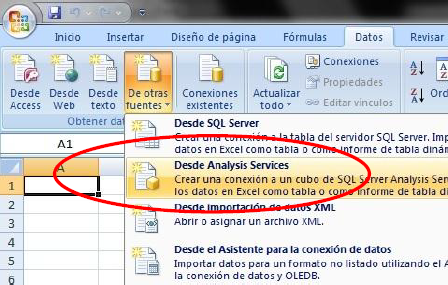
\includegraphics[scale=0.7]{Rips1}
\label{fig:Rips1}
\\ \textbf{Fuente:} Propia.
\end{figure}\\\\
2. A continuación se despliega una caja de diálogo para establecer la conexión a la base de datos que contiene el respectivo reporte (ver gráfica 2), a continuación se deben diligenciar los campos de conexión de la siguiente manera:\\
a. Nombre del servidor : cubos.sispro.gov.co.\\
b. Credenciales de conexión: se debe seleccionar la segunda opción “Utilizar el nombre de usuario y la contraseña siguientes”.Nombre de usuario: sispro.local(usuario) (usuario debe reemplazarlo por el usuario asignado por el administrador del SGD)
Contraseña: colocar la respectiva contraseña.
Diligenciados estos datos, se debe dar clic en la opción “Siguiente”.\\
\begin{figure}[h]
\centering
\caption{Opción de Analysis Services} 
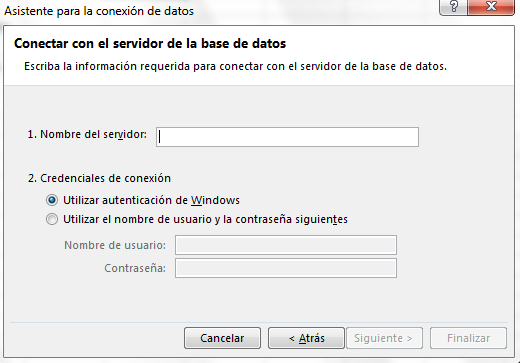
\includegraphics[scale=0.7]{Rips2}
\label{fig:Rips2}
\\ \textbf{Fuente:} Propia.
\end{figure}\\\\
3. A continuación se despliega una nueva caja de diálogo en la que se podrá selección el reporte a consultar (ver Gráfica 3), entonces en la opción “Seleccione la base de datos que contiene la información que desee”, seleccione “Cubos –SGD”, a continuación fíjese que la opción “Conectar con una tabla o a un cubo específico” este activa, tal y como se puede observar en la Gráfica 3.\\
A continuación se presenta un ejemplo de conexión para el Cubo de Aportes a la protección Social:\\
Al desplegarse los cubos disponibles o a los que se tiene acceso, seleccione el reporte identificado como “Per – Prestación Servicios de Salud”. Para seguir avanzando de clic en la opción “Siguiente”\\

\begin{figure}[h]
\centering
\caption{Conexión de datos} 
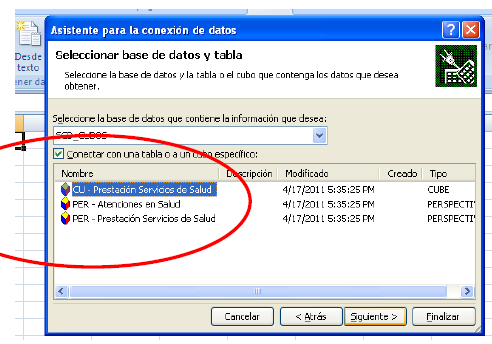
\includegraphics[scale=0.7]{Rips3}
\label{fig:Rips3}
\\ \textbf{Fuente:} Propia.
\end{figure}

4. A continuación se desplegará la pantalla que se muestra en la Gráfica, en la cual al lado izquierdo se muestra el panel de navegación para ejecutar las diferentes consultas sobre el reporte y el cual contiene las medidas y dimensiones para su navegación.

\begin{figure}[h]
\centering
\caption{Tabla } 
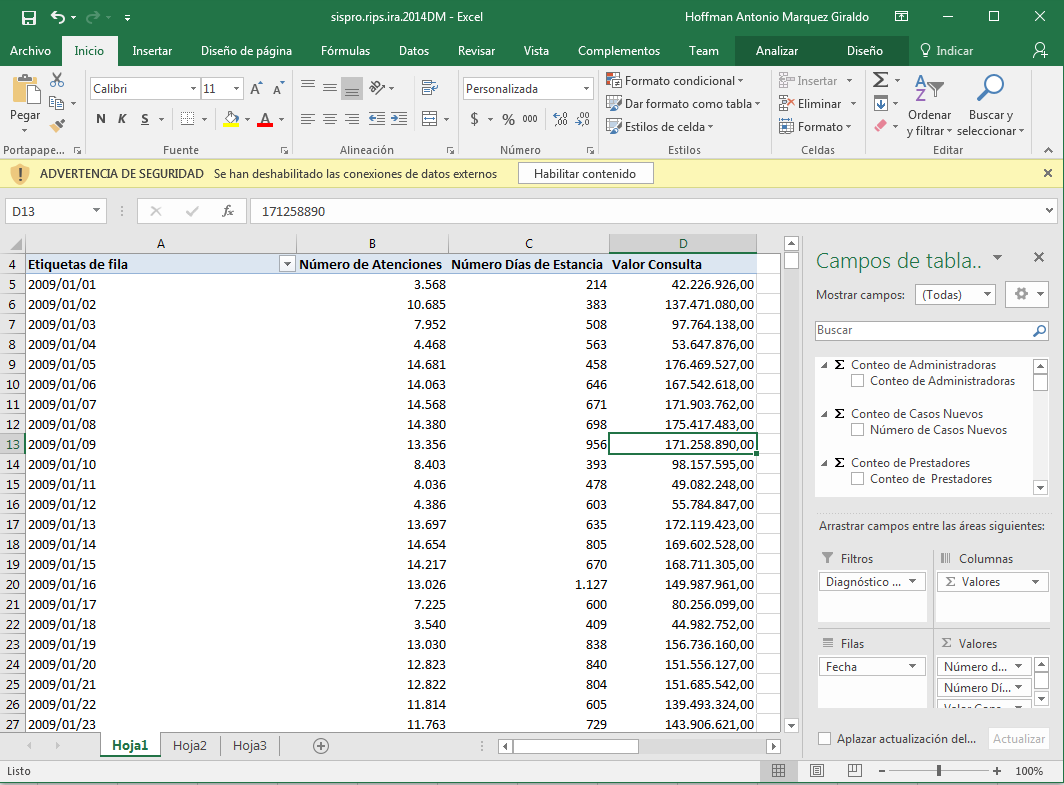
\includegraphics[scale=0.3]{Rips4}
\label{fig:Rips4}
\\ \textbf{Fuente:} Propia.
\end{figure}


\subsection{Instituto Nacional de Salud}


1. Al igual que en la anterior explicación realizada para obtener los datos del hospital del sur a través de la fuente de información (CUBO)se selecciona la Opción de Sivigila para tener acceso a la información por parte del Instituto Nacional de salud.

\begin{figure}[h]
\centering
\caption{Acceso a SIVIGILA} 
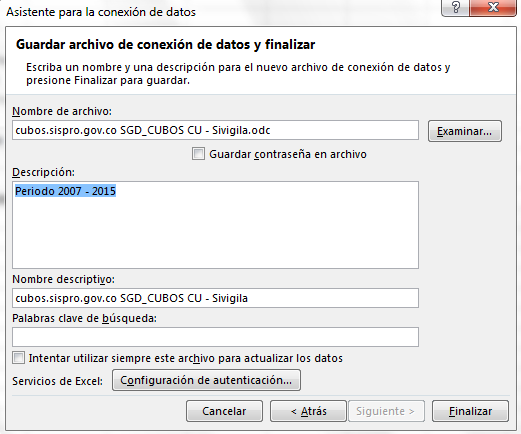
\includegraphics[scale=0.4]{Rips6}
\label{fig:Rips6}
\\ \textbf{Fuente:} Propia.
\end{figure}
2. Para terminar con el proceso para poder acceder a la información, se selecciona finalizar.
\begin{figure}[h]
\centering
\caption{Finalizar} 
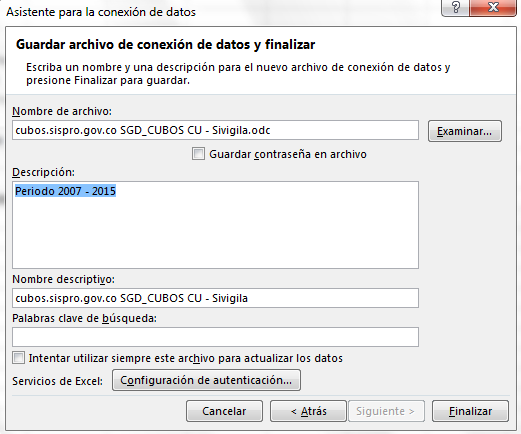
\includegraphics[scale=0.7]{Rips6}
\label{fig:Rips16}
\\ \textbf{Fuente:} Propia.
\end{figure}



\subsection{Secretaría Distrital de Medio Ambiente}
1.Para acceder a Dicha información por parte de la Red de Monitoreo de Calidad del Aire de Bogotá (RMCAB)se puede hacer de manera directa a la dirección : http://201.245.192.252:81/ en los link  “Publicaciones/Informes Anuales” y “Publicaciones/Informes Trimestrales y Semestrales” y en la página del Observatorio Ambiental de Bogotá,  en el link de aire. - See more at: \
%http://ambientebogota.gov.co/red-de-calidad-del-aire#sthash.kwnJsI4H.dpuf
\begin{figure}[h]
\centering
\caption{Reportes} 
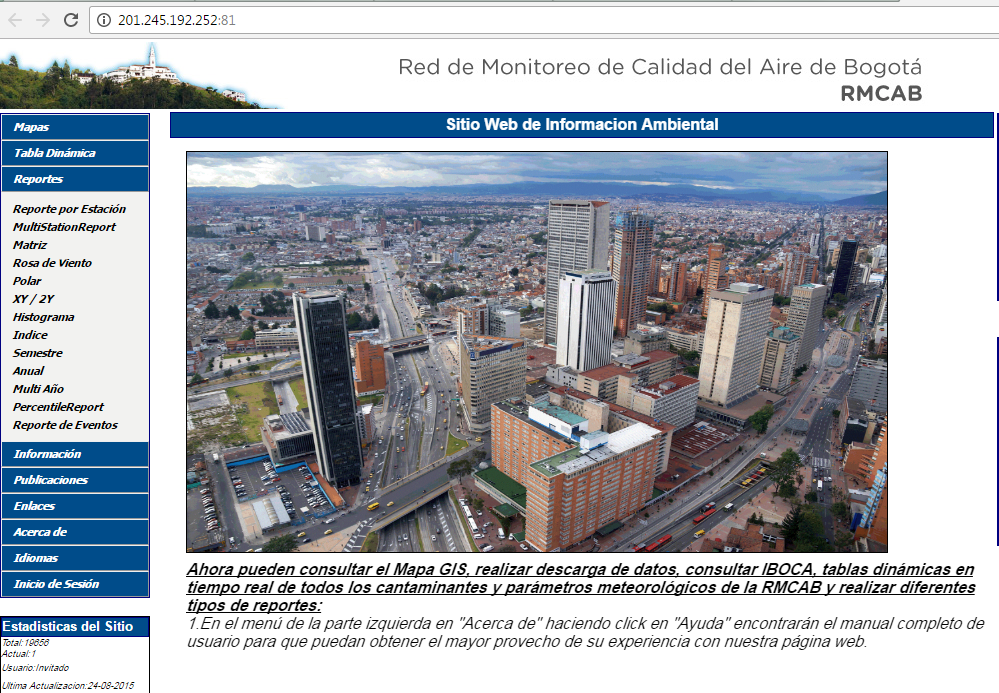
\includegraphics[scale=0.5]{RMCAB}
\label{fig:RMCAN1}
\\ \textbf{Fuente:} Propia.
\end{figure}
2. Para el caso de las estaciones de monitoreo





\section{Minería de Datos}

\begin{enumerate}
	\item \textbf{Preparación de datos:}
    \begin{enumerate}
		\item Evaluación de los datos:
        Explicación de los pasos y con captura de pantallas.
    	\item Verificación de los datos:
        Explicación de los pasos y con captura de pantallas.
    	\item Verificación de la necesidad de anonimización de los datos:
        Explicación de los pasos y con captura de pantallas.
	\end{enumerate}
    \item \textbf{Selección de datos:}
    \begin{enumerate}
		\item Caracterización de  las variables de cada una de las bases de datos,tanto los RIPS como SIVIGILA y el RMCAB: Explicación de los pasos y con captura de pantallas.
    	\item Identificación del tipo de algoritmo o técnica a realizar de minería de datos para cada base de datos: Explicación de los pasos y con captura de pantallas.
	\end{enumerate}
    \item \textbf{Modelo Inicial de Minería de Datos}
     \begin{enumerate}
		\item Diseñar las técnicas de minería de datos para cada una de las bases de datos: Explicación de los pasos y con captura de pantallas.
	\end{enumerate}
    \item \textbf{Implementación del modelo:}
      \begin{enumerate}
		\item Aplicar el modelo definidos para la minería de datos a la información original: Explicación de los pasos y con captura de pantallas.
    	\item Dar a conocer los resultados: Explicación de los pasos y con captura de pantallas.
	\end{enumerate}
\end{enumerate}

\section{Perturbación}
Para los datos de tipo entero o númericos se aplicó la distribución Gaussiana o Normal, para la alteración de sus valores y para las cadenas el intercambio de posición, de esta manera se garantizará la anonimización de los datos.
    
    \subsection{Perturbación de Datos}

\begin{enumerate}
	\item Selección de los datos a perturbar: Explicación de los pasos y con captura de pantallas.
    \item Desarrollo de los Scripts en Python: Explicación de los pasos y con captura de pantallas.
    \item Ejecución de los scripts: Explicación de los pasos y con captura de pantallas.
    \item Verificación de la correcta ejecución: Explicación de los pasos y con captura de pantallas.
\end{enumerate}

	 \subsection{Protocolo SSL}
\begin{enumerate}
	\item Búsqueda e instalación de OpenSSL\footnote{https://www.openssl.org/source/} de manera local:\\
En el buscador de Internet se ingresa al siguiente link https://www.openssl.org/source/ , en el cual se buscará la versión 1.1.0 que actualmente es la más estable según la documentación de la herramienta Fig. 4.?.

\begin{figure}[h]
\centering
\caption{Búsqueda y Descarga de OpenSSL diferente a Mac OS X} 
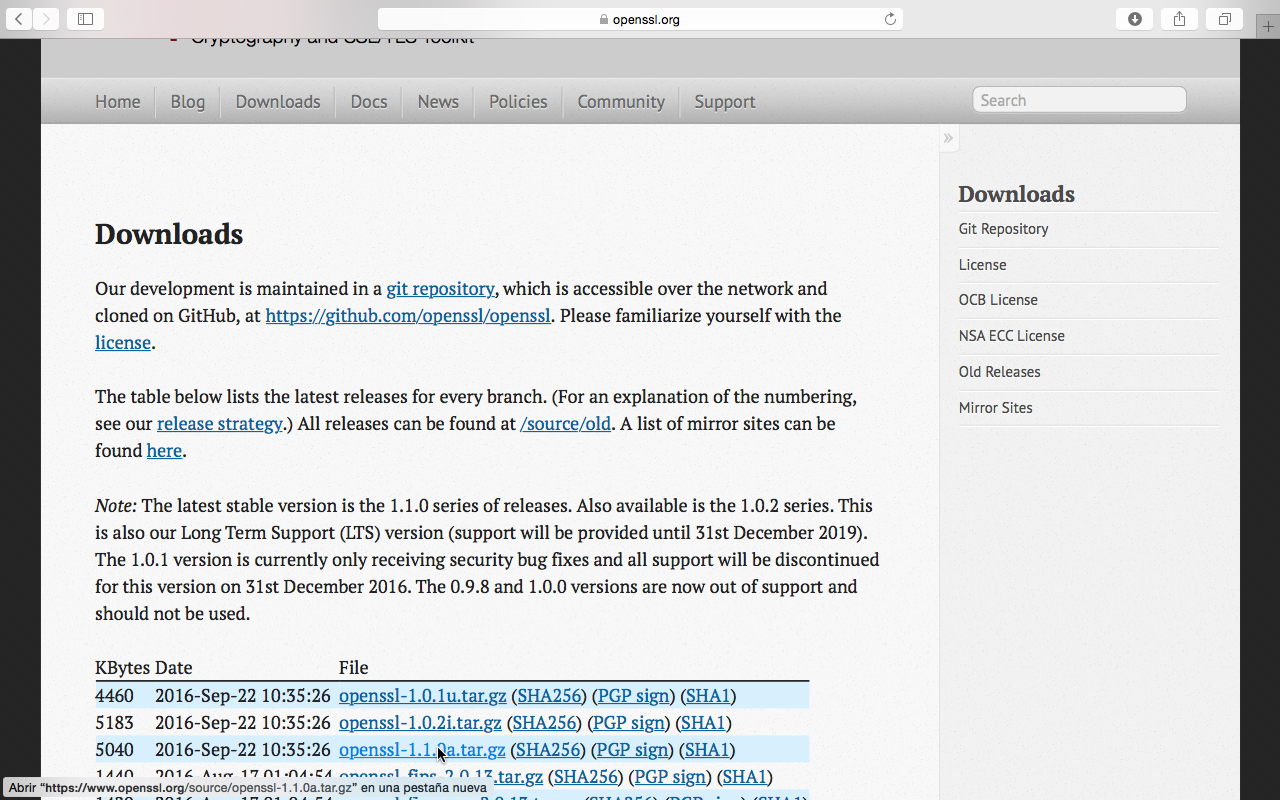
\includegraphics[scale=0.3]{1_OpenSSL}
\label{fig:1_OpenSSL}
\\ \textbf{Fuente:} Propia.
\end{figure}

Se abre un terminal en el equipo, para descargar el paquete Fig. 4.?.
\begin{figure}[h]
\centering
\caption{Descarga del paquete desde Terminal} 
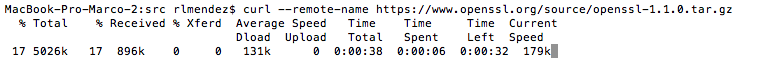
\includegraphics[scale=0.7]{2_OpenSSL}
\label{fig:2_OpenSSL}
\\ \textbf{Fuente:} Propia.
\end{figure}

Extraer el archivo y pasar a la carpeta Fig 4.?.
\begin{figure}[h]
\centering
\caption{Extracción Paquete OpenSSL} 
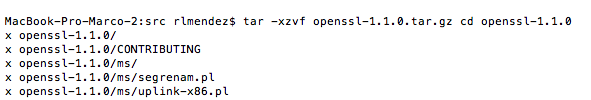
\includegraphics[scale=0.7]{3_OpenSSL}
\label{fig:3_OpenSSL}
\\ \textbf{Fuente:} Propia.
\end{figure}

Compilar e instalar según la Fig. 4.?.
\begin{figure}[h]
\centering
\caption{Instalación Paquete OpenSSL} 
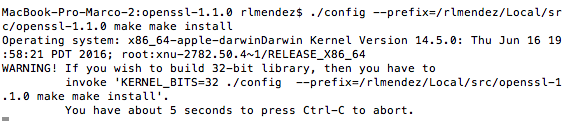
\includegraphics[scale=0.6]{4_OpenSSL}
\label{fig:4_OpenSSL}
\\ \textbf{Fuente:} Propia.
\end{figure}

Crear un vínculo simbólico que apunte según Fig. 4.?.
\begin{figure}[!htbp]
\centering
\caption{Apuntador hacía el Paquete OpenSSL} 
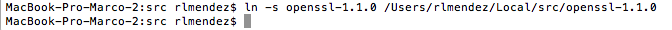
\includegraphics[scale=0.5]{5_OpenSSL}
\label{fig:5_OpenSSL}
\\ \textbf{Fuente:} Propia.
\end{figure}

Actualizar el Bash según Fig. 4.?.
\begin{figure}[!htbp]
\centering
\caption{Actualización de Bash} 
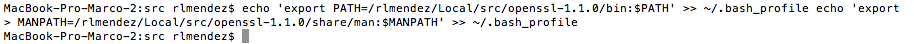
\includegraphics[scale=0.46]{6_OpenSSL}
\label{fig:6_OpenSSL}
\\ \textbf{Fuente:} Propia.
\end{figure}

Cargar las nuevas configuraciones según Fig. 4.?.
\begin{figure}[!htbp]
\centering
\caption{Cargar nuevas configuraciones} 
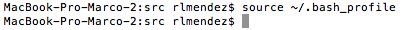
\includegraphics[scale=0.5]{7_OpenSSL}
\label{fig:7_OpenSSL}
\\ \textbf{Fuente:} Propia.
\end{figure} \\

Ejecutar las siguientes líneas para instalar los certificados según Fig. 4.?.
XXXXXXXXXXXX FALTA XXXXXXXX

Comprobar la correcta instalación según Fig. 4.?.
\begin{figure}[!htbp]
\centering
\caption{Comprobación Instalación OpenSSl} 
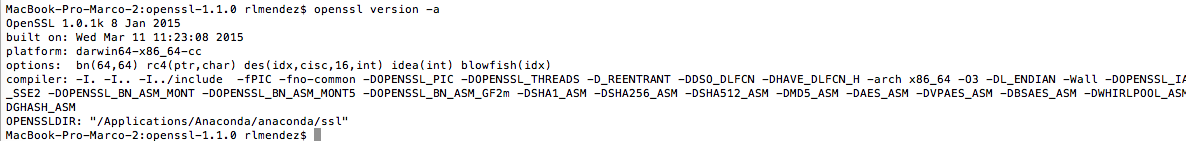
\includegraphics[scale=0.37]{9_OpenSSL}
\label{fig:9_OpenSSL}
\\ \textbf{Fuente:} Propia.
\end{figure}


    
    \item Instalación de OpenSSL en otro computador: Explicación de los pasos y con captura de pantallas.
    \item Ejecución del Protocolo mediante OpenSSL entre los dos computadores: Explicación de los pasos y con captura de pantallas.
    \item Verificar los resultados: Explicación de los pasos y con captura de pantallas.
\end{enumerate}

\clearpage

\begin{center}
 \chapter{RESULTADOS}\label{cap.resultados}
\end{center}
\section{Resultados de los procesos de Minería de Datos (Datos Originales)}
\section{Resultados de los procesos de Minería de Datos (Datos Anonimizados)}
\clearpage

\begin{center}
 \chapter{ANÁLISIS}\label{cap.analisis}
\end{center}
\section{Comparación Datos Originales - Anonimizados}
\clearpage

\begin{center}
 \chapter{CONCLUSIONES Y RECOMENDACIONES}\label{cap.conclusiones}
\end{center}

\section{Conclusiones}


\section{Recomendaciones}

\clearpage

\begin{center}
 \chapter{GLOSARIO DE TÉRMINOS}\label{cap.glosario}
\end{center}
AGENTES ETIOLOGICOS: el agente etiologico es el que causa la enfermedad. el agente transmisor es el que lo transmite de un organismo a otra.\\\\
ALGORITMO: es un conjunto prescrito de instrucciones o reglas bien definidas, ordenadas y finitas que permite realizar una actividad mediante pasos sucesivos. \\\\
ANONIMIZAR: es la necesidad de los cibernautas de ocultar información mientras navegan para evitar el uso de sus datos personales (como la dirección IP o la situación geográfica) con fines estadísticos, publicitarios o vandálicos ha causado la aparición del neologismo anonimizar, que se ha extendido después a otros ámbitos.  \\\\
DATASETS: es una colección de datos habitualmente tabulada.En general y en su versión más simple, un conjunto de datos corresponde a los contenidos de una única tabla de base de datos o una única matriz de datos estadística, donde cada columna de la tabla representa una variable en particular, y cada fila representa a un miembro determinado del conjunto de datos en cuestión. Un conjunto de datos contiene los valores para cada una de las variables, como por ejemplo la altura y el peso de un objeto, que corresponden a cada miembro del conjunto de datos. Cada uno de estos valores se conoce con el nombre de dato. El conjunto de datos puede incluir datos para uno o más miembros en función de su número de filas.\\\\
ENCRIPTACIÓN: es el proceso para volver ilegible información considera importante. La información una vez encriptada sólo puede leerse aplicándole una clave. Se trata de una medida de seguridad que es usada para almacenar o transferir información delicada que no debería ser accesible a terceros.\\\\
INFECCIÓN DE RESPIRACIÓN AGUDA: la Infección Respiratoria Aguda (IRA) constituyen un grupo de enfermedades que se producen en el aparato respiratorio, causadas por diferentes microorganismos como virus y bacterias, que comienzan de forma repentina y duran menos de 2 semanas.
La mayoría de estas infecciones como el resfriado común son leves, pero dependiendo del estado general de la persona pueden complicarse y llegar a amenazar la vida, como en el caso de las neumonías. \\\\
MORBILIDAD:es la proporción de personas (o animales) que se enferman en un sitio y tiempo determinado.1 Minoritariamente también se usa como sinónimo morbilidad, que etimológicamente es correcto.  \\\\
MORTALIDAD:indica el número de fallecimientos de una población en concreto por cada 1000 habitantes, durante un período de tiempo determinado, este puede ser durante un año. \\\\
SCRIPTS: son programas, usualmente pequeños o simples, para realizar generalmente tareas muy específicas. Los scripts son un conjunto de instrucciones generalmente almacenadas en un archivo de texto que deben ser interpretados línea a línea en tiempo real para su ejecución.\\\\
\clearpage

\begin{center}
 \chapter{REFERENCIAS}\label{cap.referencias}
\end{center}

\begin{enumerate}
	\item PLAN DE DESARROLLO INSTITUCIONAL 2013-2016 Versión Enero 2013 del Hospital del Sur.
	\item HERRANZ Javier NIN Jordi Secure and efficient anonymization of distributed confidential databases, Springer-Verlag Berlin Heidelberg 2014, Online: 23 April 2014. Int. J. Inf. Secur. (2014) 13:497–512.
	\item PENCHALAIAH PhD, SESHADRI  PhD. Effective Comparison and Evaluation of DES and Rijndael Algorithm (AES), International Journal on Computer Science and Engineering Vol. 02, No. 05, 2010, 1641-1645.
    \item CORREGIR ESTE ERROR% ÁNGEL A. Juan, SEDANO Máximo, VILA Alicia.} %<http://www.uoc.edu/in3/emath/docs/Distrib_Normal.pdf> [citado en Septiembre 18 del 2016].
    \item M. Berry, G. Linoff, “Mastering data mining: the art andscience of customer relationship management“. West Susex:John Wiley \& Sons, 1999.
    \item DAMGARD Ivan, et at. Multiparty Computation from Somewhat Homomorphic Encryption, International Association for Cryptologic Research 2012, R. Safavi-Naini and R. Canetti (Eds.): CRYPTO 2012, LNCS 7417.
    \item GHODOSI Hossein Ghodosi, et at. Multi-party computation with conversion of secret sharing, Springer Science+Business Media, LLC 2011, Des. Codes Cryptogr. (2012) 62:259–272, Online: 10 May 2011.
    \item KIRAZ SABIR Mehmet, UZUNKOL Osmanbey. Efficient and verifiable algorithms for secure outsourcing of cryptographic computations, Springer-Verlag Berlin Heidelberg 2015, Int. J. Inf. Secur, Online: 15 Nov 2015.
    \item LAUD Peeter. Privacy-Preserving Minimum Spanning Trees through Oblivious Parallel RAM for Secure Multiparty Computation, Online: 25 Nov 2014.
    \item Dirección de Regulación, Planeación, Estandarización y Normalización DIRPEN. Lineamientos para la Anonimización de microdatos VERSIÓN: 01 29-08-2014.
    \item SSL Information and FAQ [En línea] <http://info.ssl.com/article.aspx?id=10241> [citado en 18 de Septiembre del 2016].
    \item Utilizar el protocolo SSL <http://www.4d.com/docs/CMS/CMS02064.HTM> [En línea] [citado en 18 de Septiembre del 2016].
    \item SEJWANI Sapna, TANWAR Sarvesh, Implementation of X.509 Certificate for Online Applications, International Journal of Research in Advent Technology, Vol.2, No.3, March 2014, E-ISSN: 2321-9637.
    \item CELINA Drovandi. CRIPTOGRAFÍA
SEGURIDAD EN ESQUEMAS DE FILE TRANSFER SEGURIDAD EN INTERNET Revista de la Universidad de Mendoza, 2015
    \item Dr. Bhadresh P. Patel, Vishal R. Pancholi. Enhancement of Cloud Computing Security with Secure Data Storage using AES IJIRST –International Journal for Innovative Research in Science and Technology Volume 2 Issue 09 February 2016 ISSN (online): 2349-601.
    \item GOMEZ Vieitis Alvaro. Sistema seguros de acceso y transmisión de datos, RA-MA Editorial.
    \item VELASCO Sánchez Paola Maritza, ANÁLISIS DE LOS MECANISMOS DE ENCRIPTACIÓN PARA LA SEGURIDAD DE LA INFORMACIÓN EN REDES DE COMUNICACIONES, FACULTAD DE INGENIERÍA MAESTRÍA EN REDES DE COMUNICACIONES, PONTIFICIA UNIVERSIDAD CATÓLICA DEL ECUADOR Año 2015
    \item Weiss, S.M. y Indurkhya, N. “Predictive Data Mining. A Practical Guide”Morgan Kaufmann Publishers, San Francisco, 1998.
    \item Cabena, P., Hadjinian, P., Stadler, R., Verhees, J. Y Zanasi, A. “Discovering Data Mining. From Concept to Implementation”, Prentice Hall, 1998.
    \item DAN Goodin.Poorly anonymized logs reveal NYC cab drivers’ detailed whereabouts [En linea]. New York: Dirección URL: <http://arstechnica.com/tech-policy/2014/06/poorly-anonymized-logs-reveal-nyc-cab-drivers-detailed-whereabouts/>. [30, Marzo 2015].
    \item HERNANDEZ Alexander New York taxi details can be extracted from anonymised data, researchers say [En linea]. New York: Dirección URL: <https://www.theguardian.com/technology/2014/jun/27/new-york-taxi-details-anonymised-data-researchers-warn>. [30, Marzo 2015].
    \item Constitución Política de Colombia Bogotá Colombia Leyer 1991.
    \item CUARTAS Rodriguez E, JALLER Escudero JD. El Habeas Data como Derecho fundamental y la Ley 1581 de 2012 y su decreto 1377 de 2013-2014
    \item Congreso de la República de Colombia Ley 1712 de 2014.
    \item ONU United Nations Statistical Commission. Fundamental principles of official statistics. Off Rec Econ Soc Counc. 1994.
    \item Unión Europea UE. Europeas C, de la Unión Europea C. Directiva 95/46/CE del Parlamento Europeo y del Consejo de 24 de octubre de 1995 relativa a la protección de las personas físicas en lo que respecta al tratamiento de datos personales ya la libre circulación de estos datos. Agencia de Protección de Datos; 1997.
\end{enumerate}


\begin{center}
 \chapter{ANEXOS}\label{cap.anexos}
\end{center}

\end{document}

-